\begin{apendicesenv}

\partapendices

\chapter{Detalhamento das Expressões de Busca elaboradas }
\label{ExpressoesdeBusca}

Neste apêndice é apresentado o detalhamento das expressões de busca elaboradas para o levantamento de características apresentado no apêndice \ref{Levantamento de características-apendice}.


O raciocínio usado para a construção das Strings de pesquisa é apresentado a seguir :

\begin{enumerate}
\item Definir uma subquestão de pesquisa:

		\textbf{Quais seriam as características relevantes na escolha de um determinado CMS levando em consideração um contexto específico?}
		
\item Separar palavras chaves:

\textbf{CMS , características, atributos }

\item Elaborar a \textit{String} de Busca com base nas palavras chaves:

\textbf{(“Content manager system “ OR “CMS” OR “Sistema gerenciador de conteudo”) AND (“features” OR “attributes” OR “appearance”)}

\item Submeter a \textit{String} de Busca em alguma base de dados conhecida: 
 \begin{itemize}
 \item IEEE;
 \item ACM;
 \item Science Direct;
 \item Springer
 \item Scopus
 \end{itemize}
 
\item Refinar a String de Pesquisa caso a quantidade de artigos retornados seja superior a 60.
\end{enumerate}

Para o teste das Expressões de Busca foi escolhida a base de dados IEEE, pois a IEEE oferece inúmeros filtros que facilitam o refinamento da Expressão de Busca, conforme a necessidade.

\section{Resultados para os CMS mais populares}
 
Após a aplicação da \textit{String} de Pesquisa na base de dados IEEE foram obtidos os seguintes resultados:

\textbf{(“Content manager system “ OR “CMS” OR “Sistema gerenciador de conteudo”) AND (“features” OR “attributes” OR “appearance”)} foram retornados 545.871 resultados.

Para refinar a String de pesquisa foram adicionados os CMSs mais populares gerando uma nova String de Pesquisa

\textbf{(“Content manager system“ OR “CMS” OR “Sistema gerenciador de conteudo”) AND (“features” OR “attributes” OR “appearance”) AND (“Wordpress”  OR  “Joomla” OR “Drupal”)}

Aplicando-se a String de pesquisa novamente na base de dados IEEE foram obtidos 999 resultados.

Dentre esses resultados foi observado que muitos artigos encontrados não estavam relacionados com CMS, nem se quer com computação, sendo assim a String de pesquisa foi ajustada para:

\textbf{(“Content AND manager AND system “ OR “CMS” OR “Sistema gerenciador de conteudo”) AND (“features” OR “attributes” OR “appearance”)} resultando em 58 resultados.



Após a aplicação dos critérios de exclusão da seção X restaram 32 artigos.
		
Porém para o levantamento de características não bastou apenas considerar somente os CMSs mais populares, foi necessário confrontar características de CMSs não populares para o estudo. Então foi criada uma nova string de pesquisa para filtrar artigos que tivessem o foco de CMSs não populares.

 \section{Resultados para os CMS não populares}
 \label{resultados_nao_populares}

Para esta etapa foi feita uma nova String de pesquisa que exclui os CMS populares e acrescenta a característica \textit{open source}. 

("CMS" OR "Content Management System") NOT “Wordpress”   NOT   “Joomla”  NOT “Drupal” AND (" features"  AND "open source")

Após a aplicação constatou-se 715 resultados considerando todo o texto, abstract e título.Porém o resultado não foi satisfatório e o filtro de apenas abstract e título do \textit{Advanced Search } do IEEE foi ativado mudando a quantidade de resultados para apenas 8. Um resultado considerado satisfatório.

Nessa fase os critérios de seleção apresentados na seção \ref{CExclusion} foram mantidos e dois artigos dos 8 selecionados foram descartados.

Porém mais um teste foi feito trocando-se a palavra \textit{features} na String de pesquisa por \textit{appearance} a fim de levantar mais artigos para a pesquisa e a  nova String: 

(("CMS" OR "Content Management System") NOT “Wordpress” NOT “Joomla” NOT “Drupal” AND (" appearance" AND "open source")) retornou 97 resultados.

O que não foi satisfatório. Como solução foi aplicado o filtro \textit{Publication Year}do próprio IEEE considerando apenas artigos dos anos de 2010 a 2014 e assim a quantidade de arquivos retornados caiu para 49.

Dos 49 artigos investigados apenas 6 artigos foram selecionados com a aplicação dos critérios de exclusão da seção \ref{CExclusion}.


\section{Critérios de Exclusão para os artigos selecionados}
\label{CExclusion}

A partir dos 58 artigos selecionados foram definidos critérios de exclusão para uma melhor seleção de características, sendo assim foram excluidos:

\begin{itemize}
\item Artigos que não mencionavam em seu título ou abstract a palavra CMS, ou \textit{Content Management System}, ou Drupal, ou Wordpress ou Joomla, ou demais palavras relacionadas.
\item Artigos fechados.
\item Não apresentar, ou não deixar claro no texto a existência de pelo menos 5 características de CMSs.

\end{itemize}

\begin{landscape}
\chapter{Levantamento de Características de CMS - Tabelas}
\label{Levantamento de características-apendice}

\section{Contexto de artigos Lidos}

\subsection{Contexto para artigos envolvendo CMSs mais populares}


	\begin{longtable}{|p{10pt}|p{320pt}|p{315pt}|}
 	\caption{Contexto para artigos levantados.} \label{tabela_contexto}\\
 	\hline
 	 {\raggedright \textbf{Id}}
 	 & {\raggedright \textbf{Título}}
 	 & {\raggedright \textbf{Contexto}}\\
 	\hline
 	 {\raggedright 1}
 	 & {\raggedright Comparativo de Ferramentas de Criação e Gestão de Web Sites CMS (Content Management System).}
 	 & {\raggedright Desenvolvimento do Web Site do Tribunal de Contas do Estado do Pará. \cite{costa}}\\
 	\hline
 	 {\raggedright 2}
 	 & {\raggedright WordPress as Library CMS.}
 	 & {\raggedright Criação de uma biblioteca virtual usando WordPress.\cite{jones_2011} }\\
 	\hline
 	 {\raggedright 3} 
 	 & {\raggedright Uma Prospecção de Plataformas para o Desenvolvimento do Sistema
 	 “Todos Nós em Rede”.}
& {\raggedright Construção de uma rede social para professores com o objetivo de apoiar a comunicação e a práticas profissionais do dia a dia. \cite{Reis}
}\\
 	\hline
 	 {\raggedright 4}
 	 & {\raggedright Building Computer System for Musical School
 	 with CSM Plone.}
 	 & {\raggedright Construção de um sistema para uma escola de música usando o CMS Plone.\cite{gadja}} \\
 	\hline
 	{\raggedright 5}
 	 & {\raggedright Joomla. Drupal and WordPress - A Statistical
 	 Comparison of Open Source CMS.}
 	 & {\raggedright Testar o desempenho de 3 CMS escolhidos: Caso 1: montagem de página com adição de plugins. Caso 2 : mesmo caso 1 só que com ambiente diferenciado.\cite{patel}} \\
 	\hline
 	{\raggedright 6}
 	 & {\raggedright Comparative analysis of web security in open source content management system.}
 	 & {\raggedright Testar a segurança de 3 CMS escolhidos: Caso 1- Criar páginas comuns e submeter tais páginas a ataques WEB ex: SQL injection. No caso 2 foi utilizado Acunetix WVS Reporter v6.0 para descobrir o potencial de segurança em diferentes CMS.\cite{Patel2013}} \\
 	\hline
 	{\raggedright 7}
 	 & {\raggedright Using {Content} {Management} {System} {Joomla}! to {Build} a {Website} for {Research} {Institute} {Needs}.}
 	 & {\raggedright Alteração de Templates no Jommla.\cite{Xiang2010}} \\
 	\hline
 		{\raggedright 8}
 	 	 & {\raggedright Optimization model of management and security of multimedia content using {Drupal} {CMS}.}
 	 	 & {\raggedright Uso do Drupal para a construção de sites com segurança para multimídia \cite{Ennert2012}} \\
 	 	\hline
 	 	
 		{\raggedright 9}
 	 	 & {\raggedright The {Web} {Development} {Based} on the {Drupal} {System}.}
 	 	 & {\raggedright Apresentação de características do drupal e desenvolvimento de um website em seguida.\cite{Cheng2012}} \\
 	 	\hline
 	 	
 	 		{\raggedright 10}
 	 	 	 & {\raggedright Role of {Content} {Management} {Software} ({CMS}) in libraries for information dissemination}.
 	 	 	 & {\raggedright Utilização do CMS Joomla para a construção de uma biblioteca virtual.\cite{Patnaik2015}} \\
 	 	 	\hline
 	 	 	
 	 	 		{\raggedright 11}
 	 	 	 	 & {\raggedright Software {Development} for {Cloud}: {An} {Experiential} {Study}.}
 	 	 	 	 & {\raggedright Desenvolvimento em nuvem usando CMS.\cite{Marimuthu2013}} \\
 	 	 	 	\hline
	{\raggedright 12}
 	 & {\raggedright Virtual-learning content management system for problem-based learning ({PBL}) courses.}
 	 & {\raggedright Sistema baseado em CMS para o ensino de PBL.\cite{AbuKasim2012}} \\
 	\hline
 	
 		{\raggedright 13}
 	 	 & {\raggedright {NEIMiner}: {A} model driven data mining system for studying environmental impact of nanomaterials.}
 	 	 & {\raggedright Sistema de mineração de dados usando o CMS Drupal.\cite{Tang2012}} \\
 	 	\hline
 	 	
 	 	{\raggedright 14}
 	 	 	 	 & {\raggedright A game with a purpose for annotating {Greek} folk music in a web content management system.}
 	 	 	 	 & {\raggedright Sistema para hospedagem de música e protótipo de jogo.\cite{Giouvanakis2013}} \\
 	 	 	 	\hline
 	 	 	 	
 	 	 	 	
 	 	 {\raggedright 15}
 	 	  	 	 & {\raggedright Designing of e-commerce system by {CMS} {Joomla} software.}
 	 	  	 	 & {\raggedright Utilização do joomla para a construção de um site para e-commerce.\cite{Dorosh2009}} \\
 	 	  	 	\hline
 	 	  	 	
 	 	  	 	{\raggedright 16}
 	 	  	 & {\raggedright Realization of electronic textbook by means of {Drupal} {Content} {Management} {System}.}
 	 	  	 	 	 	 	 	 & {\raggedright Uso do CMS Drupal para a produção de livros eletronicos.\cite{Iliev2013}} \\
 	 	  	 	 	 	 	 	\hline
 	 	  	 	
 	 	  	 {\raggedright 17}
 	 	  	  	 	   	 	 & {\raggedright The development of a new branch of the economy: e-commerce. {Practical} use with {Content} {Management} {Systems} {Joomla}! and enlargement {VirtueMart}.}
 	 	  	  	 	   	 	 & {\raggedright Uso do Joomla para a construção de um site de e-commerce.\cite{Hetka2009}} \\
 	 	  	  	 	   	 	\hline	
 	 	  	 	
 	 	  	 	
 	 	  	 	{\raggedright 18}
 	 	  	 	 	 	 & {\raggedright Exploring possibilities to analyse microblogs for dependability information in variability-intensive open source software systems. }
 	 	  	 	 	 	 & {\raggedright Utilização de microblogs para análise de confiabilidade de sistemas de software livre.\cite{Galster2013}} \\
 	 	  	 	 	 	\hline
 	 	  	 	 	 	
 	 	  
 	 	   
 	 	   {\raggedright 19}
 	 	    	 	 & {\raggedright Extending web content management systems navigation capabilities with semantic navigation maps.}
 	 	    	 	 & {\raggedright Técnicas de recuperação de informação em CMS.\cite{Distante2010}} \\
 	 	    	 	\hline
 	 	    	 	
 	 	    	 	
 	 	  {\raggedright 20}
 	 	   	 	 & {\raggedright Integrating social web and e-learning to enhance cooperation in the building sector.}
 	 	   	 	 & {\raggedright Criação de uma Plataforma de Aprendizagem Colaborativa.\cite{Longo2014}} \\
 	 	   	 	\hline
 	{\raggedright 21}
  	 	  	 & {\raggedright Security in {Drupal}.}
  	 	  	 	 	 	 	 	 & {\raggedright Segurança no Drupal. \cite{Kumar2014}} \\
  	 	  	 	 	 	 	 	\hline
  	 	  	 	
  	 	  	 {\raggedright 22}
  	 	  	  	 	   	 	 & {\raggedright Integration of captivate and {JOOMLA}: {Online} demonstration and assessment {eLearning} resources.}
  	 	  	  	 	   	 	 & {\raggedright Integração do Joomla com o Adobe captive em uma plataforma web para ensino multimídia.\cite{Aw2010}} \\
  	 	  	  	 	   	 	\hline	
  	 	  	 	
  	 	  	 	
  	 	  	 	{\raggedright 23}
  	 	  	 	 	 	 & {\raggedright A {Multi}-sites {Scheme} {Based} on {Open} {Source} {CMS}, {Drupal}. }
  	 	  	 	 	 	 & {\raggedright Uso de Drupal para construção de sistemas multi-Locais.\cite{Jinwei2010}} \\
  	 	  	 	 	 	\hline
  	 	  	 	 	 	
  	 	  
  	 	   
  	 	   {\raggedright 24}
  	 	    	 	 & {\raggedright Content server for use in {Power} {Electronics} courses.}
  	 	    	 	 & {\raggedright Implementação de um portal web para auxílio de estudantes. \cite{Serdio2010}} \\
  	 	    	 	\hline
  	 	    	 	
  	 	    	 	
  	 	  {\raggedright 25}
  	 	   	 	 & {\raggedright Drupal {Content} {Management} {System} on {Mobile} {Phone}.}
  	 	   	 	 & {\raggedright Construindo um site com auxílio do drupal para tecnologia mobile.\cite{Nurminen2008}} \\
  	 	   	 	\hline
  	 	   	 	
	{\raggedright 26}
 	 	  	 & {\raggedright An {API} for {Quran} portal using {Drupal} technology.}
 	 	  	 	 	 	 	 	 & {\raggedright Uso do Drupal para desenvolvimento de aplicação em nuvem. \cite{Adhoni2014}} \\
 	 	  	 	 	 	 	 	\hline
 	 	  	 	
 	 	  	 {\raggedright 27}
 	 	  	  	 	   	 	 & {\raggedright Learning 2.0 in the {Information} {Systems} {Curriculum}.}
 	 	  	  	 	   	 	 & {\raggedright Criação de um sistema para aprendizagem com o auxílio do Drupal.\cite{Albrecht2009}} \\
 	 	  	  	 	   	 	\hline	
 	 	  	 	
 	 	  	 	
 	 	  	 	{\raggedright 28}
 	 	  	 	 	 	 & {\raggedright Supporting {Agricultural} {Communities} with {Workflows} on {Heterogeneous} {Computing} {Resources}. }
 	 	  	 	 	 	 & {\raggedright Solução web para comunidades agrícolas envolvendo grand e processamento de dados\cite{Balasko2014}} \\
 	 	  	 	 	 	\hline
 	 	  	 	 	 	
 	 	  
 	 	   
 	 	   {\raggedright 29}
 	 	    	 	 & {\raggedright Automatically classifying and interpreting polar datasets with {Apache} {Tika}.}
 	 	    	 	 & {\raggedright Extração de meta dados em sistema para a análise de ambiente na antartida.\cite{Burgess2014}} \\
 	 	    	 	\hline
 	 	    	 	
 	 	    	 	
 	 	  {\raggedright 30}
 	 	   	 	 & {\raggedright Advanced solution for delivering educational multimedia content based on content management system.}
 	 	   	 	 & {\raggedright Aplicação multimidia usando o Drupal.\cite{Cymbalak2012}} \\
 	 	   	 	\hline
	{\raggedright 31}
 	 	  	 & {\raggedright My-{Plant}.org: {A} phylogenetically structured social network.}
 	 	  	 	 	 	 	 	 & {\raggedright Criação de uma rede social com auxílio de Drupal.\cite{Hanlon2010}} \\
 	 	  	 	 	 	 	 	\hline
 	 	  	 	
 	 	  	 {\raggedright 32}
 	 	  	  	 	   	 	 & {\raggedright {eAssessment} in {English} for specific purposes.}
 	 	  	  	 	   	 	 & {\raggedright Estudo de caso para construir de um sistema de avaliação para alunos de nível superior.
 	 	  	  	 	   	 	 .\cite{Polic2014}} \\
 	 	  	  	 	   	 	\hline	
 	 	  	 	
 	 	  	 	
 	 	  	 	{\raggedright 33}
 	 	  	 	 	 	 & {\raggedright Mobile interface to content management system based on {HTML}5 and {Drupal}: {A} case study. }
 	 	  	 	 	 	 & {\raggedright Fornecer conteúdo multimídia para dispositivos móveis.\cite{Priya2012}} \\
 	 	  	 	 	 	\hline
 	 	  	 	 	 	
 	 	  
 	 	   
 	 	   {\raggedright 34}
 	 	    	 	 & {\raggedright Talkoot software appliance for collaborative science.}
 	 	    	 	 & {\raggedright Construção de Rede Social.\cite{Ramachandran2009}} \\
 	 	    	 	\hline
 	 	    	 	
 	 	    	 	
 	 	  {\raggedright 35}
 	 	   	 	 & {\raggedright A {Semantic} {Web} {Approach} in the {Implementation} of a {Linked} {Data} {Portal} {Using} a {CMS}.}
 	 	   	 	 & {\raggedright Construção de um framework envolvendo web semantica.\cite{Giannopoulou2014}} \\
 	 	   	 	\hline
	{\raggedright 36}
 	 	  	 	 	 	 & {\raggedright Hacking is not random: a case-control study of webserver-compromise risk. }
 	 	  	 	 	 	 & {\raggedright Fatores de risco do uso de cms em web services. \cite{Vasek2015}} \\
 	 	  	 	 	 	\hline
 	 	  	 	 	 	
 	 	  
 	 	   
 	 	   {\raggedright 37}
 	 	    	 	 & {\raggedright Microblogging in {Open} {Source} {Software} {Development}: {The} {Case} of {Drupal} and {Twitter}.}
 	 	    	 	 & {\raggedright Twwiter e Drupal.\cite{Wang2014}} \\
 	 	    	 	\hline
 	 	    	 	
 	 	    	 	
 	 	  {\raggedright 38}
 	 	   	 	 & {\raggedright{QR}-code generator.}
 	 	   	 	 & {\raggedright Gerador de QR Codes.\cite{Sutheebanjard2010}} \\
 	 	   	 	\hline
	{\raggedright 39}
 	 	  	 & {\raggedright A case study on the use of community platforms for inter-enterprise innovation.}
 	 	  	 	 	 	 	 	 & {Projeto de pesquisa para a implementação de um sistema para um ambiente corporativo.\cite{Larrinaga2011}} \\
 	 	  	 	 	 	 	 	\hline
 	 	  	 	
 	 	  	 {\raggedright 40}
 	 	  	  	 	   	 	 & {\raggedright Modelling remote laboratories integrations in e-learning tools through remote laboratories federation protocols.}
 	 	  	  	 	   	 	 & {\raggedright Laboratorios remotos educativos.\cite{Orduna2012}} \\
 	 	  	  	 	   	 	\hline	
 	 	  	 	
 	 	  	 	
 	 	  	 	{\raggedright 41}
 	 	  	 	 	 	 & {\raggedright Generic integration of remote laboratories in learning and content management systems through federation protocols. }
 	 	  	 	 	 	 & {\raggedright Laboratorios remotos educativos.\cite{Orduna2013}} \\
 	 	  	 	 	 	\hline
 	 	  	 	 	 	
 	 	   	 	 	 	   	 		 	  	 	
 	\end{longtable}
 	
\subsection{Contexto para artigos envolvendo CMSs não populares}
\begin{longtable}{|p{10pt}|p{320pt}|p{315pt}|}
 	\caption{Contexto para artigos levantados CMSs não populares.} 
 	\label{tabela_contexto_não_populares}\\
 	\hline
 	 {\raggedright \textbf{Id}}
 	 & {\raggedright \textbf{Título}}
 	 & {\raggedright \textbf{Contexto}}\\
 	\hline
 	 {\raggedright 1}
 	 & {\raggedright 
 	 Content management system : Comparative case study.}
 	 & {\raggedright Estudo de Caracteríticas em CMSs Open source. \cite{Nath_Arora}}\\
 	\hline
 	 {\raggedright 2}
 	 & {\raggedright A {Customized} {Open} {Source} {Content} {Management} {System} to {Support} {Collaborative} {Distance} {Learning}: {The} {J}@{LON} {Platform}.}
 	 & {\raggedright Sistema para ensino a distancia com auxilio de zope plone.\cite{Staccini2007} }\\
 	\hline
 	 {\raggedright 3} 
 	 & {\raggedright An {Open} {Source} {Approach} for a {Military} {Situational} {Awareness} {System}An {Open} {Source} {Approach} for a {Military} {Situational} {Awareness} {System}.}
& {\raggedright Discussão de falhas em sistema militares. Sistemas que envolvem o uso de CMS. \cite{Loechel2012}
}\\
 	\hline
 {\raggedright 4}
 	 & {\raggedright 
 	 Automated notification and document downloading in {E}-learning - development of an agent-based framework utilizing the push-pull technology interaction policy.}
 	 & {\raggedright Sistema para E-learning utilizando CMS.
 	  \cite{Latif2008}}\\
 	\hline
 	 {\raggedright 5}
 	 & {\raggedright Construction of education application platform based on {Plone} content management system.}
 	 & {\raggedright Construção de uma aplicação educacional com o auxílio de zope plone.\cite{Jiugen2012} }\\
 	\hline
 	 {\raggedright 6} 
 	 & {\raggedright An {Open} {Source} {Approach} for a {Military} {Situational} {Awareness} {System}An {Open} {Source} {Approach} for a {Military} {Situational} {Awareness} {System}.}
& {\raggedright Construção de sistema para e-commerce. \cite{Kiatruangkrai2010}
}\\
 	\hline
 {\raggedright 7}
 	 & {\raggedright 
 	 Content management system for web portal.}
 	 & {\raggedright Informações básicas sobre CMS para um portal web.\cite{Nakwaski2010}}\\
 	\hline
 	 {\raggedright 8}
 	 & {\raggedright The {Construction} of {Virtual} {Reference} {Advisory} {Platform} {Based} {Plone} {Content} {Management} {System}.}
 	 & {\raggedright Utilização do plone para construção de sistema de aconselhamento virtual.\cite{Lina2010}}\\
 	\hline
 	 {\raggedright 9} 
 	 & {\raggedright A {Web}-based {CMS}/{PDM} {Integration} for {Product} {Design} and {Manufacturing}.}
& {\raggedright Aplicação prática para integrar CMS e PDM (Product Data Management). \cite{Yen2008}
}\\
 	\hline 
{\raggedright 10}
 	 & {\raggedright 
 	{LearnSquare}: {Thai} open-source {Learning} {Management} {System}.}
 	 & {\raggedright Ilustrar as carcterísticas do sistema LearnSquare.\cite{Mekpiroon2008}}\\
 	\hline
 	 {\raggedright 11}
 	 & {\raggedright A hybrid architecture for developing an educational {Content} {Management} {System}.}
 	 & {\raggedright Reutilização e gerenciamento de conteudo educacional usando CMS e LMS.\cite{Vasques2011}}\\
 	\hline
 	 {\raggedright 12} 
 	 & {\raggedright The visual wiki for the first step of {KMS} in community college.}
& {\raggedright Explorando fatores de sucesso em CMSs no contexto de sistemas para aprendizagem. \cite{Yusoff2011}
}\\
 	\hline 	
\end{longtable} 	

\clearpage	
\section{Características de CMSs mais populares}

	\begin{longtable}{|p{10pt}|p{220pt}|p{415pt}|}
 	\caption{Características de CMSs levantadas para CMSs populares.} 
 	\label{caracteristicas_CMS}\\
 	\hline
 	 {\raggedright \textbf{Id}}
 	 & {\raggedright \textbf{Característica}}
 	 & {\raggedright \textbf{Descrição}}\\
 	\hline
 	{\raggedright {1}}
 	 	 & {\raggedright {Facilidade de instalação}}
 	 	 & {\raggedright {Ato de transferir os arquivos baixados para o  sistema operacional, realizar as devidas configurações e executar o programa instalado em
 	 	 uma maquina local. \cite{costa}}}\\
 	 	\hline
 	{\raggedright {2}}
 	 	 & {\raggedright {Usabilidade}}
 	 	 & {\raggedright {Facilidade com que as pessoas podem
 	 	 empregar uma ferramenta ou objeto a fim de realizar uma tarefa específica e importante. \cite{costa}}}\\
 	 	\hline
 	{\raggedright {3}}
 	 	 & {\raggedright {Flexibilidade}}
 	 	 & {\raggedright {Ter os recursos necessários para evoluir de acordo com suas funcionalidades. \cite{Reis} }}\\
 	 	\hline
 	 	{\raggedright {4}}
 	 	 	 	 & {\raggedright {Segurança da ferramenta}}
 	 	 	 	 & {\raggedright {Gerenciamento de segurança, incluindo gerenciamento de sessão
 	 	 	 	 e controle de acesso baseado em função de conteúdos / operações. \cite{Distante2010}}}\\
 	 	 	 	\hline
 	 {\raggedright {5}}
 	  	 	 	 	 & {\raggedright {Interatividade}}
 	  	 	 	 	 & {\raggedright {Processo bem organizado de criação de conteúdos.\cite{Iliev2013}}}\\
 	  	 	 	 	\hline
 	  	 	 	 	
 	 {\raggedright {6}}
 	  	 	 	 	 & {\raggedright {Suporte a serviços mobiles( Smathphones, tablets)}}
 	  	 	 	 	 & {\raggedright {Permitir o uso do CMS em dispositivos mobiles como smarthphones e tablets \cite{Jones}}}\\
 	  	 	 	 	\hline
 	 {\raggedright {7}}
 	  	 	 	 	 & {\raggedright {Documentação}}
 	  	 	 	 	 & {\raggedright {Apresentar guia de instalação, guia de início rápido, tutoriais, wikis, fóruns de discussão de desenvolvedores, entre outros. \cite{Reis}}}\\
 	  	 	 	 	\hline
 	 {\raggedright {8}}
 	  	 	 	 	 & {\raggedright {Conformidade com os padrões World Wide Web Consortium}}
 	  	 	 	 	 & {\raggedright {Conformidade com padrões para a criação e interpretação de conteúdos para WeB \cite{Reis}
 	  	 	 	 	  }}\\
 	  	 	 	 	\hline
 	  	 	 	 	{\raggedright {9}}
 	  	 	 	 	 & {\raggedright {Taxonomia}}
 	  	 	 	 	 	 	 	 	 & {\raggedright {Forma com que os CMS organizam seu conteúdo. O Joomla por exemplo define a organização de seu conteúdo em "seções" e "categorias". \cite{costa} }}\\
 	  	 	 	 	 	 	 	 	\hline 
 	 {\raggedright {10}}
 	  	 	 	 	 & {\raggedright {Liberdade para alteração de um template específico}}
 	  	 	 	 	 & {\raggedright {O usuário tem liberdade para editar, ou acrescentar conteúdo em um determinado template. \cite{Reis}}}\\
 	  	 	 	 	\hline	 	 	 	
{\raggedright {11}}
 	 	 & {\raggedright {Configuração para interagir com outros sites}}
 	 	 & {\raggedright {Possuir a capacidade para se comunicar com outras páginas web. \cite{Reis} }}\\
 	 	\hline
 	{\raggedright {12}}
 	 	 & {\raggedright {Edição de conteúdo em qualquer aplicativo (como o Dreamweaver ou Word) sem ter que mover o conteúdo do servidor para o desktop}}
 	 	 & {\raggedright {O conteúdo pode ser editado diretamente em qualquer outro software (Word, Dreamweaver), sem a necessidade de download para o desktop \cite{gadja}}}\\
 	 	\hline
 	{\raggedright {13}}
 	 	 & {\raggedright {Existência de recursos para controle de acesso}}
 	 	 & {\raggedright {Controlar o acesso a informações individuais e dados com base em papéis definidos, grupos de usuários. (Definição de quais usuários ou grupos de usuários podem visualizar, editar, publicar
 	 	 dados individuais, etc} \cite{Ennert2012}}\\
 	 	\hline
 	 	{\raggedright {14}}
 	 	 	 	 & {\raggedright {Permitir upload de uma quantidade grande de tipos de arquivos (Word, Excel, RTF, PDF)}}
 	 	 	 	 & {\raggedright {Disponibilização de vários tipos de arquivos no conteúdo da página. \cite{gadja}}}\\
 	 	 	 	\hline
 	 {\raggedright {15}}
 	  	 	 	 	 & {\raggedright {Permitir o gerenciamento de conteúdo de qualquer navegador( Até os de celular)}}
 	  	 	 	 	 & {\raggedright {Acesso ao CMS por qualquer browser. Até browsers de dispositivos móveis como tablets e smarthphones \cite{gadja}}}\\
 	  	 	 	 	\hline
 	  	 	 	 	
 	 {\raggedright {16}}
 	  	 	 	 	 & {\raggedright {Facilidade em criar novos conteúdos}}
 	  	 	 	 	 & {\raggedright {A criação de conteúdos deve ocorrer sem qualquer habilidade com linguagens de programação. \cite{gadja}}}\\
 	  	 	 	 	\hline
 	 {\raggedright {17}}
 	  	 	 	 	 & {\raggedright {Boa capacidade para realizar pesquisas, buscas}}
 	  	 	 	 	 & {\raggedright {Suporte para uso simples, armazenamento, pesquisa e dados
 	  	 	 	 	 recuperação por critérios diferentes e filtros.} \cite{Ennert2012}}\\
 	  	 	 	 	\hline
 	 {\raggedright {18}}
 	  	 	 	 	 & {\raggedright {Existência de Templates e Plugins disponíveis para a alteração do site em questão}}
 	  	 	 	 	 & {\raggedright {O CMS eve dispor de temas para a modificação do seu Layout e plugins para a adição de funcionalidades.\cite{gadja}}}\\
 	  	 	 	 	\hline
 	  	 	 	 	{\raggedright {19}}
 	  	 	 	 	 & {\raggedright {Os dados podem ser acessados ou armazenados em bancos de dados relacionais}}
 	  	 	 	 	 & {\raggedright {Os dados podem ser armazenados, ou acessados a partir de bancos de dados relacionais. Exemplos:
 	  	 	 	 	  Oracle, SQLServer, PostgreSQL,
 	  MySQL, Interbase, e bancos de dados compatíveis com ODBC. \cite{gadja}}}\\
 	  	 	 	 	 	 	 	 	\hline 
 	 {\raggedright {20}}
 	  	 	 	 	 & {\raggedright {Tempo de carregamento da página}}
 	  	 	 	 	 & {\raggedright {Em ms (milisegundos)\cite{patel}}}\\
 	  	 	 	 	\hline
{\raggedright {21}}
 	 	 & {\raggedright {Tamanho da Página}}
 	 	 & {\raggedright {Tamanho total da página em KB. \cite{patel}}}\\
 	 	\hline
 	{\raggedright {22}}
 	 	 & {\raggedright {Total de Requisições}}
 	 	 & {\raggedright {Número de requisições enviadas ao servidor ao se carregar uma página. \cite{patel}}}\\
 	 	\hline
 	{\raggedright {23}}
 	 	 & {\raggedright {Total de arquivos JS}}
 	 	 & {\raggedright {Número de arquivos \textit{Java Script} usados pelo CMS para fazer uma página. \cite{patel}}}\\
 	 	\hline
 	 	{\raggedright {24}}
 	 	 	 	 & {\raggedright {Total de arquivos CSS}}
 	 	 	 	 & {\raggedright {Número de arquivos CSS usados pelo CMS para fazer uma página. \cite{patel}}}\\
 	 	 	 	\hline
 	 {\raggedright {25}}
 	  	 	 	 	 & {\raggedright {Tempo em que se armazena o conteúdo na memória cache antes da página carregar}}
 	  	 	 	 	 & {\raggedright {Chamado de PLT.\cite{patel}}}\\
 	  	 	 	 	\hline
 	  	 	 	 	
 	 {\raggedright {26}}
 	  	 	 	 	 & {\raggedright {Quantidade de dados armazenados na memória cache antes da página carregar}}
 	  	 	 	 	 & {\raggedright {Chamado de PS \cite{patel}}}\\
 	  	 	 	 	\hline
 	 {\raggedright {27}}
 	  	 	 	 	 & {\raggedright {Existência de recursos de proteção a ataques do tipo SQL Injection}}
 	  	 	 	 	 & {\raggedright {Tipo de ataque à segurança web no qual o atacante adiciona código SQL através da caixa de entrada de formulário web para ganhar acesso aos dados e realizar mudanças. \cite{Patel2013}}}\\
 	  	 	 	 	\hline
 	 {\raggedright {28}}
 	  	 	 	 	 & {\raggedright {Existência de recursos de proteção a ataques do tipo XXS}}
 	  	 	 	 	 & {\raggedright {Forma de ataque por meio de conteúdos dinâmicos (gifs, banners, entre outros.) que disparam scripts maliciosos, roubam \textit{cookies}, ou enviam solicitações de conteúdo não autorizado.\cite{Patel2013}}}\\
 	  	 	 	 	\hline
 	  	 	 	 	{\raggedright {29}}
 	  	 	 	 	 & {\raggedright {Existência de recursos de proteção a ataques do tipo Remote File Inclusion RFI}}
 	  	 	 	 & {\raggedright {Com auxilio de um arquivo remoto normalmente chamado de SHELL, o \textit{hacker}  pode obter
 	  	 	 	 direitos de administrador do servidor. A shell é um arquivo interface gráfica do usuário
 	  	 	 	  que é usado para visitar os arquivos remotos e executar
 	  seu próprio código em servidores da web.\cite{Patel2013} }}\\
 	  	 	 	 	 	 	 	 	\hline 
 	 {\raggedright {30}}
 	  	 	 	 	 & {\raggedright {Existência de recursos de proteção a ataques do tipo LFI}}
 	  	 	 	 	 & {\raggedright {\textit{Local File Inclusion} é uma forma de ataque que consiste em  incluir arquivos em um servidor através do navegador web. \cite{Patel2013})}}\\
 	  	 	 	 	\hline
{\raggedright {31}}
 	 	 & {\raggedright {Existência de recursos de proteção a ataques do tipo Directory Transversal}}
 	 	 & {\raggedright {Método de invasão no qual os \textit{hackers} se baseiam em ataques de passagem de diretório para tentar o acesso a arquivos do servidor Web de acesso restrito e que estão fora do diretório raiz. \cite{Patel2013} }}\\
 	 	\hline
 	{\raggedright {32}}
 	 	 & {\raggedright {Existência de recursos de proteção a ataques do tipo  \textit{Cookie Poisoning}}}
 	 	 & {\raggedright {Ataques de \textit{Cookie Poisoning}  envolvem a modificação do conteúdo de um \textit{cookie} (informações pessoais armazenadas no computador de um usuário da Web), a fim de contornar os mecanismos de segurança. Usando ataques de envenenamento de cookie, os atacantes podem obter informações não autorizadas sobre outro usuário e roubar sua identidade \cite{Imperva}.}}\\
 	 	\hline
 	{\raggedright {33}}
 	 	 & {\raggedright {Existência de recursos de proteção a ataques do tipo \textit{Cross-Site Request Forgery (CSRF)}}}
 	 	 & {\raggedright {É um ataque que força um usuário autenticado em uma página web a  executar ações indesejadas \cite{Owasp} }}\\
 	 	\hline
 	 	{\raggedright {34}}
 	 	 	 	 & {\raggedright {Ser software Livre ou não}}
 	 	 	 	 & {\raggedright {O CMS é open source ou proprietário. Preocupação com o licenciamento do CMS. \cite{Cheng2012}}}\\
 	 	 	 	\hline
 	 {\raggedright {35}}
 	  	 	 	 	 & {\raggedright {Popularidade}}
 	  	 	 	 	 & {\raggedright {Popularidade do CMS. O conceito popularidade é explicado na seção \ref{popularidade_CMS}}}\\
 	  	 	 	 	\hline
 	  	 	 	 	
 	 {\raggedright {36}}
 	  	 	 	 	 & {\raggedright {Taxa de atualização}}
 	  	 	 	 	 & {\raggedright {Frequencia com que o CMS oferece atualizações incorporando novos recursos e sistemas de apoio. \cite{Iliev2013} }}\\
 	  	 	 	 	\hline
 	 {\raggedright {37}}
 	  	 	 	 	 & {\raggedright {Tamanho da Comunidade}}
 	  	 	 	 	 & {\raggedright {Apoio da comunidade para a solução de problemas. Desenvolvedores contribuem para a evolução e manutenção do CMS.  \cite{Cheng2012} }}\\
 	  	 	 	 	\hline
 	 {\raggedright {38}}
 	  	 	 	 	 & {\raggedright {Simplicidade de acesso}}
 	  	 	 	 	 & {\raggedright {Os dados em um CMS podem ser definidos de várias formas, sem muitas restrições, facilitando o acesso. \cite{Ennert2012}}}\\
 	  	 	 	 	\hline
 	  	 	 	 	{\raggedright {39}}
 	  	 	 	 	 & {\raggedright {Existência de recursos para vários idiomas}}
 	  	 	 	 	 	 	 	 	 & {\raggedright {Suporte a vários idiomas distintos. \cite{Ennert2012}}}\\
 	  	 	 	 	 	 	 	 	\hline 
 	 {\raggedright {40}}
 	  	 	 	 	 & {\raggedright Existência de recursos para gerência de versões de conteúdo}
 	  	 	 	 	 & {\raggedright {Controle de versão, atualizações e revisões. \cite{Ennert2012}}}\\
 	  	 	 	 	\hline
{\raggedright {41}}
 	 	 & {\raggedright {Permitir suporte para conteúdos multimídia}}
 	 	 & {\raggedright {Visualizar, partilhar, catalogar e permitir gestão de conteúdo multímidia (vídeos, fotos, músicas)}\cite{Ennert2012}}\\
 	 	\hline
 	{\raggedright {42}}
 	 	 & {\raggedright {Modularidade}}
 	 	 & {\raggedright {Quebra de funcionalidades por meio de várias extensões diferentes. \cite{Iliev2013} }}\\
 	 	\hline
 	{\raggedright {43}}
 	 	 & {\raggedright {Permitir  interação com várias ferramentas}}
 	 	 & {\raggedright {O CMS pode ser usado em conjunto com diversas ferramentas. Exemplos: Frameworks, sistemas operacionais, bancos de dados, entre outros. \cite{Nurminen2008}}}\\
 	 	\hline
 	 	{\raggedright {44}}
 	 	 	 	 & {\raggedright {Custo}}
 	 	 	 	 & {\raggedright {Redução de custos com o desenvolvimento local e com manutenção. \cite{Iliev2013}}}\\
 	 	 	 	\hline
 	 {\raggedright {45}}
 	  	 	 	 	 & {\raggedright {Manutenção}}
 	  	 	 	 	 & {\raggedright {Melhorias na manutenção evitando duplicação de conteúdo. \cite{Iliev2013}}}\\
 	  	 	 	 	\hline
 	  	 	 	 	
 	 {\raggedright {46}}
 	  	 	 	 	 & {\raggedright {Ser Multiplataforma}}
 	  	 	 	 	 & {\raggedright {Capacidade de se adaptar a diversos tipos de sistemas. Exemplos: mobiles, sistemas operacionais. \cite{Nurminen2008}}}\\
 	  	 	 	 	\hline
 	 {\raggedright {47}}
 	  	  	 	 	 	 & {\raggedright {Fácil Utilização}}
 	  	  	 	 	 	 & {\raggedright {Sem conhecimento de programação web é possível criar um site em um curto período de tempo. \cite{Patnaik2015}}}\\
 	  	  	 	 	 	\hline
 	 {\raggedright {48}}
 	  	 	 	 	 & {\raggedright {Não requer conhecimento de Linguagem de Programação para uso}}
 	  	 	 	 	 & {\raggedright {Não é necessário o conhecimento de linguagens de programação para a criação de um web site. \cite{Distante2010}}}\\
 	  	 	 	 	\hline
 	 {\raggedright {49}}
 	  	 	 	 	 & {\raggedright {Variabilidade}}
 	  	 	 	 	 & {\raggedright {Grande quantidade de módulos, plugins, templates e outros recursos. \cite{Galster2013}}}\\
 	  	 	 	 	\hline
 	  	 	 	 	{\raggedright {50}}
 	  	 	 	 	 & {\raggedright {Confiabilidade}}
 	  	 	 	 	 	 	 	 	 & {\raggedright {Probabilidade da
 	  	 	 	 	 	 	 	 	 operação de um software estar livre de falhas por um período determinado
 	  	 	 	 	 	 	 	 	 de tempo em um ambiente específico. \cite{Galster2013}}}\\
 	  	 	 	 	 	 	 	 	\hline 
 	 {\raggedright {51}}
 	  	 	 	 	 & {\raggedright {Modificabilidade}}
 	  	 	 	 	 & {\raggedright {Capacidade de prover recursos para modificar o site em questão conforme a necessidade do usuário. \cite{Cymbalak2012}}}\\
 	  	 	 	 	\hline
{\raggedright {52}}
 	 	 & {\raggedright {Extensibilidade}}
 	 	 & {\raggedright {O CMS pode ser extendido por meio de seus modulos. \cite{Ennert2012}}}\\
 	 	\hline
 	{\raggedright {53}}
 	 	 & {\raggedright {Ciclo de desenvolvimento rápido (Rad)}}
 	 	 & {\raggedright {Adaptação ao Ciclo de Desenvolvimento Rápido (RAD). \cite{Hanlon2010}}}\\
 	 	\hline
 	{\raggedright {54}}
 	 	 & {\raggedright {Arquitetura flexivel e extensivel}}
 	 	 & {\raggedright {A arquitetura é modularizada e fácimente extensível. \cite{Hanlon2010}}}\\
 	 	\hline
 	 	{\raggedright {55}}
 	 	 	 	 & {\raggedright {Capacidade de Reuso}}
 	 	 	 	 & {\raggedright {Módulos do CMS podem ser reutilizados conforme a necessidade do desenvolvedor. \cite{Priya2012}}}\\
 	 	 	 	\hline
 	 {\raggedright {56}}
 	  	 	 	 	 & {\raggedright {Mecanismo anti phishing}}
 	  	 	 	 	 & {\raggedright {Mecanismo contra fraudes, na qual o fraudador tenta adquirir dados pessoais, como senhas, dados financeiros, por meio de SMS, emails entre outros. \cite{Vasek2015}}}\\
 	  	 	 	 	\hline
 	  	 	 	 	
 	 {\raggedright {57}}
 	  	 	 	 	 & {\raggedright {Violação de segurança por redirecionamento de página}}
 	  	 	 	 	 & {\raggedright {Uma quebra de segurança pode ocorrer quando ao clicar em um determinado link ocorre um direcionamento de página. \cite{Vasek2015} }}\\
 	  	 	 	 	\hline

	\end{longtable}

\section{Características de CMSs não populares}
\begin{longtable}{|p{10pt}|p{220pt}|p{430pt}|}
 	\caption{Características de CMSs levantadas para CMSs não populares.} 
 	\label{caracteristicas_CMS_não_popular}\\
 	\hline
 	 {\raggedright \textbf{Id}}
 	 & {\raggedright \textbf{Característica}}
 	 & {\raggedright \textbf{Descrição}}\\
 	\hline
 	{\raggedright {1}}
 	 	 & {\raggedright {Geração automática de Interface de Usuário}}
 	 	 & {\raggedright {Interface com o usuário é gerada automaticamente. \cite{Nath_Arora}}}\\
 	 	\hline
 	{\raggedright {2}}
 	 	 & {\raggedright {Inscrição automática de usuário}}
 	 	 & {\raggedright {Permite que o usuário entre automaticamente no momento da abertura do site.}\cite{Nath_Arora}}\\
 	 	\hline
 	{\raggedright {3}}
 	 	 & {\raggedright {Controle dinâmico}}
 	 	 & {\raggedright {Permitir a manipulação dos dados fornecidos \cite{Nath_Arora}}}\\
 	 	\hline
 	 	{\raggedright {4}}
 	 	 	 	 & {\raggedright {Notificação de senha esquecida}}
 	 	 	 	 & {\raggedright {Este recurso suporta usuários que esqueceram sua senha. O CMS notifica o usuário com uma nova senha aleatória} \cite{Nath_Arora}}\\
 	 	 	 	\hline
 	 {\raggedright {5}}
 	  	 	 	 	 & {\raggedright {Confirmação por email}}
 	  	 	 	 	 & {\raggedright {Confirma uma nova identificação de usuário (ID) para o usuário \cite{Nath_Arora}}}\\
 	  	 	 	 	\hline
 	  	 	 	 	
 	 {\raggedright {6}}
 	  	 	 	 	 & {\raggedright {Backup}}
 	  	 	 	 	 & {\raggedright {Facilidade de backup de dados para um usuário salvar seus dados.\cite{Nath_Arora}}}\\
 	  	 	 	 	\hline
 	 {\raggedright {7}}
 	  	 	 	 	 & {\raggedright {Gerenciamento de usuários}}
 	  	 	 	 	 & {\raggedright {Gerencia as informações da dos usuários e suas respectivas autenticações.\cite{Nath_Arora}}}\\
 	  	 	 	 	\hline
 	 {\raggedright {8}}
 	  	 	 	 	 & {\raggedright {Geração automática de código}}
 	  	 	 	 	 & {\raggedright {Código da página é gerado automaticamente. \cite{Nath_Arora}}}\\
 	  	 	 	 	\hline
 	  	 	 	 	{\raggedright {9}}
 	  	 	 	 	 & {\raggedright {Permitir múltiplos usuários}}
 	  	 	 	 	 	 	 	 	 & {\raggedright {Múltiplo gerenciamento de acesso do usuário por meio de de travamento.\cite{Nath_Arora}}}\\
 	  	 	 	 	 	 	 	 	\hline 
 	 {\raggedright {10}}
 	  	 	 	 	 & {\raggedright {Permitir download de arquivos}}
 	  	 	 	 	 & {\raggedright {Gestão dos downloads de arquivos por um usuário.\cite{Nath_Arora}}}\\
 	  	 	 	 	\hline	

 {\raggedright {11}}
 	  	 	 	 	 & {\raggedright {Permitir gerenciamento de arquivos}}
 	  	 	 	 	 & {\raggedright {Gestão dos arquivos enviados pelo usuário.\cite{Nath_Arora}}}\\
 	  	 	 	 	\hline
 	 {\raggedright {12}}
 	  	 	 	 	 & {\raggedright {Comentários}}
 	  	 	 	 	 & {\raggedright {Facilidade para fornecer comentários.\cite{Nath_Arora}}}\\
 	  	 	 	 	\hline
 	 {\raggedright {13}}
 	  	 	 	 	 & {\raggedright {Mecanismo anti plágio}}
 	  	 	 	 	 & {\raggedright {Permite que um site identifique se existe conteúdo plagiado em seu sistema.\cite{Nath_Arora}}}\\
 	  	 	 	 	\hline
 	  	 	 	 	{\raggedright {14}}
 	  	 	 	 	 & {\raggedright {Fóruns}}
 	  	 	 	 	 	 	 	 	 & {\raggedright {Suporte a fóruns de discussão.\cite{Nath_Arora}}}\\
 	  	 	 	 	 	 	 	 	\hline 
 	 {\raggedright {15}}
 	  	 	 	 	 & {\raggedright {Verificação de Formato}}
 	  	 	 	 	 & {\raggedright {Recurso que pode ser usado onde o conteúdo pode ser entregue em dois ou mais formatos como qualquer documento pode ser entregue em pdf ,. doc ,. tex etc. ou arquivos de mídia podem ser entregues em. avi ,. dat, etc identificação automática do formato e submetido a conversão para o formato desejado.\cite{Nath_Arora}}}\\
 	  	 	 	 	\hline
 	  	 	 	 	 	  	 	 	 	
\end{longtable}
	
\end{landscape}

\section{Cruzamento de Características de CMS com características SQuaRE}
\label{Cruzamento_Apendice}
A tabela \ref{mapeamento_Square} apresenta as características de CMS levantadas com as características relacionadas a qualidade do produto e as suas respectivas subcaracterísticas. Já a tabela \ref{mapeamento_Square_uso} apresenta o mesmo raciocínio só que sob a perspectiva de qualidade em uso.

	\begin{longtable}{|p{175pt}|p{18pt}|p{110pt}|p{120pt}|}
 	\caption{Cruzamento de características de CMS com características SQuaRE - Qualidade do Produto.} 
 	\label{mapeamento_Square}\\
 	\hline
 	 {\raggedright \textbf{Característica CMS}}
 	 & {\raggedright \textbf{Qtd}}
% 	 & {\raggedright \textbf{Conceito}}
 	 & {\raggedright \textbf{Característica SQuaRE}}
 	  	 & {\raggedright \textbf{Subcaracterística SQuaRE}}\\
 	\hline
 	{\raggedright {Ser software Livre ou não}}
 	 	 & {\raggedright {40}}
% 	 	 & {\raggedright {-----}}
 	 	 & {\raggedright {Não se aplica a SQuaRE}}
 	 	  	 	 & {\raggedright Não se aplica a SQuaRE}\\
 	 	\hline
 	{\raggedright {Facilidade para interação com várias ferramentas}}
 	 	 & {\raggedright {38}}
% 	 	 & {\raggedright {Qualidade do Produto}}
 	 	 & {\raggedright {Adequação Funcional}}
 	 	 & {\raggedright {Completude Funcional}}\\
 	 	\hline
{\raggedright {Modularidade}}
 	 	 & {\raggedright {32}}
% 	 	 & {\raggedright {Qualidade do Produto}}
 	 	 & {\raggedright {Manutenibilidade}}
 	 	 & {\raggedright {Modularidade}}\\
 	 	\hline
% {\raggedright {Facilidade para interação com várias ferramentas}}
%  	 	 & {\raggedright {28}}
%%  	 	 & {\raggedright {Qualidade do Produto}}
%  	 	 & {\raggedright {Adequação Funcional}}
%  	 	 & {\raggedright {Completude Funcional}}\\
%  	 	\hline
 {\raggedright {Os dados podem ser acessados ou armazenados em bancos de dados relacionais}}
  	 	 & {\raggedright {28}}
%  	 	 & {\raggedright {Qualidade do Produto}}
  	 	 & {\raggedright {Adequação Funcional}}
  	 	 & {\raggedright {Completude Funcional}}\\
  	 	\hline
 {\raggedright {Existência de recursos para controle de acesso}}
  	 	 & {\raggedright {25}}
%  	 	 & {\raggedright {Qualidade do Produto}}
  	 	 & {\raggedright {Segurança}}
  	 	 & {\raggedright {Autenticidade}}\\
  	 	\hline
  	{\raggedright {Existência de Templates e Plugins disponíveis para a alteração do site em questão}}
  	 	  	  & {\raggedright {19}}
  	 	%  	  & {\raggedright {------}}
  	 	  	 & {\raggedright {Não se aplica a SQuaRE}}
  	 	  	 & {\raggedright {Não se aplica a SQuaRE}}\\
  	 	  	 	\hline
  	 	  	 	
 {\raggedright {Popularidade}}
  	 	 & {\raggedright {17}}
%  	 	 & {\raggedright {------}}
  	 	 & {\raggedright {Não se aplica a SQuaRE}}
  	 	 & {\raggedright {Não se aplica a SQuaRE}}\\
  	 	\hline
 
 {\raggedright {Boa capacidade para realizar pesquisas, buscas}}
  	 	 & {\raggedright {17}}
%  	 	 & {\raggedright {Qualidade do Produto}}
  	 	 & {\raggedright {Adequação Funcional}}
  	 	 & {\raggedright {Completude Funcional}}\\
  	 	\hline
  	 	 
 {\raggedright {Configuração para interagir com outros sites}}
  	 	 & {\raggedright {16}}
%  	 	 & {\raggedright {Qualidade do Produto}}
  	 	 & {\raggedright {Adequação Funcional}}
  	 	 & {\raggedright {Completude Funcional}}\\
  	 	\hline
{\raggedright {Facilidade em criar novos conteúdos}}
  	 	 & {\raggedright {16}}
%  	 	 & {\raggedright {Qualidade do Produto}}
  	 	 & {\raggedright {Usabilidade}}
  	 	 & {\raggedright {Operacionalidade}}\\
  	 	\hline
  	 	
 {\raggedright {Interatividade}}
  	 	 & {\raggedright {15}}
%  	 	 & {\raggedright {Qualidade do Produto}}
  	 	 & {\raggedright {Usabilidade}}
  	 	 & {\raggedright {Operacionalidade}}\\
  	 	\hline
 {\raggedright {Usabilidade}}
   	 	 & {\raggedright {14}}
 %  	 	 & {\raggedright {Qualidade do Produto}}
   	 	 & {\raggedright {Usabilidade}}
   	 	 & {\raggedright {Característica Square}}\\
   	 	\hline
  {\raggedright {Segurança da Ferramenta}}
   	 	 & {\raggedright {14}}
 %  	 	 & {\raggedright {Qualidade do Produto}}
   	 	 & {\raggedright {Segurança}}
   	 	 & {\raggedright {Característica Square}}\\
   	 	\hline
 
 {\raggedright {Tamanho da Comunidade}}
  	 	 & {\raggedright {13}}
%  	 	 & {\raggedright {--------}}
  	 	 & {\raggedright {Não se aplica a SQuaRE}}
  	 	 & {\raggedright {Não se aplica a SQuaRE}}\\
  	 	\hline
 {\raggedright {Liberdade para alteração de um template específico}}
  	 	 & {\raggedright {13}}
%  	 	 & {\raggedright {Qualidade do Produto}}
  	 	 & {\raggedright {Manutenibilidade}}
  	 	 & {\raggedright {Modificabilidade}}\\
  	 	\hline
  {\raggedright {Permitir suporte para conteúdos multimídia}}
   	 	 & {\raggedright {13}}
 %  	 	 & {\raggedright {Qualidade do Produto}}
   	 	 & {\raggedright {Adequação Funcional}}
   	 	 & {\raggedright {Completude Funcional}}\\
   	 	\hline
 {\raggedright {Ser multiplataforma}}
   	 	 & {\raggedright {13}}
 %  	 	 & {\raggedright {Qualidade do Produto}}
   	 	 & {\raggedright {Portabilidade}}
   	 	 & {\raggedright {Adaptabilidade}}\\
   	 	\hline
   	 	  	 	
 {\raggedright {Permitir o gerenciamento de conteúdo de qualquer navegador( Até os de celular)}}
  	 	 & {\raggedright {12}}
%  	 	 & {\raggedright {Qualidade do Produto}}
  	 	 & {\raggedright {Portabilidade}}
  	 	 & {\raggedright {Adaptabilidade}}\\
  	 	\hline
  
 {\raggedright {Manutenção}}
  	 	 & {\raggedright {11}}
%  	 	 & {\raggedright {Qualidade do Produto}}
  	 	 & {\raggedright {Manutenibilidade}}
  	 	 & {\raggedright {Característica SQuaRE}}\\
  	 	\hline  
   	 	
 {\raggedright {Permitir upload de uma quantidade grande de tipos de arquivos (Word, Excel, RTF, PDF)}}
  	 	 & {\raggedright {10}}
%  	 	 & {\raggedright {Qualidade do Produto}}
  	 	 & {\raggedright {Adequação Funcional}}
  	 	 & {\raggedright {Completude Funcional}}\\
  	 	\hline
  	 	
  	 	{\raggedright {Existência de recursos para a gerência de versão de conteúdo}}
  	 	  	 	 & {\raggedright {10}}
  	 	%  	 	 & {\raggedright {Qualidade do Produto}}
  	 	  	 	 & {\raggedright {Adequação Funcional}}
  	 	  	 	 & {\raggedright {Completude Funcional}}\\
  	 	  	 	\hline
  	 	
  	 	 
  	{\raggedright {Modificabilidade}}
  	 	  	 	 & {\raggedright {10}}
  	 	%  	 	 & {\raggedright {Qualidade do Produto}}
  	 	  	 	 & {\raggedright {Manutenibilidade}}
  	 	  	 	 & {\raggedright {Modificabilidade}}\\
  	 	  	 	\hline
  	 	
 {\raggedright Arquitetura flexível e extensível}
  	 	  	 & {\raggedright {9}}
  	 	%  	 	 & {\raggedright {--------------}}
  	 	   & {\raggedright {Não se aplica a SQuaRE}}
  	 	   & {\raggedright {Não se aplica a SQuaRE}}\\
  	 	  	 	\hline

{\raggedright {Fácil Utilização}}
  	 	 & {\raggedright {9}}
%  	 	 & {\raggedright {Qualidade do Produto}}
  	 	 & {\raggedright {Usabilidade}}
  	 	 & {\raggedright {Operacionalidade}}\\
  	 	\hline

 {\raggedright {Gerenciamento de usuários}}
  	 	 & {\raggedright {9}}
%  	 	 & {\raggedright {Qualidade do Produto}}
  	 	 & {\raggedright {Adequação Funcional}}
  	 	 & {\raggedright {Completude Funcional}}\\
  	 	\hline

 {\raggedright {Permitir download de arquivos}}
  	 	 & {\raggedright {8}}
%  	 	 & {\raggedright {Qualidade do Produto}}
  	 	 & {\raggedright {Adequação Funcional}}
  	 	 & {\raggedright {Completude Funcional}}\\
  	 	\hline
 {\raggedright {Permitir gerenciamento de arquivos}}
  	 	 & {\raggedright {8}}
%  	 	 & {\raggedright {Qualidade do Produto}}
  	 	 & {\raggedright {Adequação Funcional}}
  	 	 & {\raggedright {Completude Funcional}}\\
  	 	\hline
{\raggedright {Taxonomia}}
  	 	 & {\raggedright {7}}
%  	 	 & {\raggedright {Qualidade do Produto}}
  	 	 & {\raggedright {Manutenibilidade}}
  	 	 & {\raggedright {Modificabilidade}}\\
  	 	\hline
 



 
{\raggedright {Facilidade de instalação}}
  	 	 & {\raggedright {7}}
%  	 	 & {\raggedright {Qualidade do Produto}}
  	 	 & {\raggedright {Portabilidade}}
  	 	 & {\raggedright {Instalabilidade}}\\
  	 	\hline
{\raggedright {Permitir múltiplos usuários}}
  	 	 & {\raggedright {6}}
  	 	 
%  	 	 & {\raggedright {Qualidade do Produto}}
  	 	 & {\raggedright {Adequação Funcional}}
  	 	 & {\raggedright {Completude Funcional}}\\
  	 	\hline
{\raggedright {Não requer conhecimento de Linguagem de Programação para uso}}
  	 	 & {\raggedright {6}}
%  	 	 & {\raggedright {--------------}}
  	 	 & {\raggedright {Usabilidade}}
  	 	 & {\raggedright {Aprendizado}}\\
  	 	\hline
  	 	
{\raggedright {Geração automática de Interface de Usuário}}
  	 	 & {\raggedright {5}}
%  	 	 & {\raggedright {Qualidade do Produto}}
  	 	 & {\raggedright {Adequação Funcional}}
  	 	 & {\raggedright {Completude Funcional}}\\
  	 	\hline

{\raggedright {Edição de conteúdo em qualquer aplicativo (como o Dreamweaver ou Word) sem ter que mover o conteúdo do servidor para o desktop}}
  	 	 & {\raggedright {5}}
%  	 	 & {\raggedright {Qualidade do Produto}}
  	 	 & {\raggedright {Adequação Funcional}}
  	 	 & {\raggedright {Completude Funcional}}\\
  	 	\hline 
 {\raggedright {Existência de recursos de proteção a ataques do tipo SQL Injection}}
  	 	 & {\raggedright {4}}
%  	 	 & {\raggedright {Qualidade do Produto}}
  	 	 & {\raggedright {Segurança}}
  	 	 & {\raggedright {Integridade}}\\
  	 	\hline

{\raggedright {Variabilidade}}
  	 	 & {\raggedright {4}}
%  	 	 & {\raggedright {----------------}}
  	 	 & {\raggedright {Adequação Funcional}}
  	 	 & {\raggedright {Completude Funcional}}\\
  	 	\hline
{\raggedright {Extensibilidade}}
  	 	 & {\raggedright {4}}
%  	 	 & {\raggedright {-------------}}
  	 	 & {\raggedright {Adequação Funcional}}
  	 	 & {\raggedright {Completude Funcional}}\\
  	 	\hline
 
{\raggedright {Backup}}
  	 	 & {\raggedright {4}}
%  	 	 & {\raggedright {Qualidade do Produto}}
  	 	 & {\raggedright {Adequação Funcional}}
  	 	 & {\raggedright {Completude Funcional}}\\
  	 	\hline

{\raggedright {Documentação}}
  	 	 & {\raggedright {3}}
%  	 	 & {\raggedright {Qualidade do Produto}}
  	 	 & {\raggedright {Usabilidade}}
  	 	 & {\raggedright {Aprendizado}}\\
  	 	\hline


{\raggedright {Tempo em que se armazena o conteúdo na memória cache antes da página carregar}}
  	 	 & {\raggedright {3}}
%  	 	 & {\raggedright {Qualidade do Produto}}
  	 	 & {\raggedright {Performance}}
  	 	 & {\raggedright {Comportamento do Tempo}}\\
  	 	\hline
{\raggedright {Quantidade de dados armazenados na memória cache antes da página carregar}}
  	 	 & {\raggedright {3}}
%  	 	 & {\raggedright {Qualidade do Produto}}
  	 	 & {\raggedright {Performance}}
  	 	 & {\raggedright {Utilização de Recursos}}\\
  	 	\hline
 
 

{\raggedright Fóruns}
  	 	 & {\raggedright {3}}
%  	 	 & {\raggedright {Qualidade do Produto}}
  	 	 & {\raggedright {Adequação Funcional}}
  	 	 & {\raggedright {Completude Funcional}}\\
  	 	\hline  	 	
{\raggedright {Suporte a serviços mobiles ( Smathphones tablets...)}}
  	 	 & {\raggedright {2}}
%  	 	 & {\raggedright {Qualidade do Produto}}
  	 	 & {\raggedright {Portabilidade}}
  	 	 & {\raggedright {Adaptabilidade}}\\
  	 	\hline
 {\raggedright {Tempo de carregamento da página}}
  	 	 & {\raggedright {2}}
%  	 	 & {\raggedright {Qualidade do Produto}}
  	 	 & {\raggedright {Eficiência de Desempenho}}
  	 	 & {\raggedright {Comportamento do tempo}}\\
  	 	\hline
 {\raggedright {Total de Requisições}}
  	 	 & {\raggedright {2}}
%  	 	 & {\raggedright {Qualidade do Produto}}
  	 	 & {\raggedright {Eficiência de Desempenho}}
  	 	 & {\raggedright {Utilização de Recursos}}\\
  	 	\hline
{\raggedright {Existência de recursos de proteção a ataques do tipo Proteção contra XXS}}
  	 	 & {\raggedright {2}}
%  	 	 & {\raggedright {Qualidade do Produto}}
  	 	 & {\raggedright {Segurança}}
  	 	 & {\raggedright {Integridade}}\\
  	 	\hline
 
 {\raggedright {Existência de recursos de proteção a ataques do tipo Cookie Poisoning}}
  	 	 & {\raggedright {2}}
%  	 	 & {\raggedright {Qualidade do Produto}}
  	 	 & {\raggedright {Segurança}}
  	 	 & {\raggedright {Integridade}}\\
  	 	\hline
{\raggedright {Existência de recursos de proteção a ataques do tipo Cross-Site Request Forgery (CSRF)}}
  	 	 & {\raggedright {2}}
%  	 	 & {\raggedright {Qualidade do Produto}}
  	 	 & {\raggedright {Segurança}}
  	 	 & {\raggedright {Integridade}}\\
  	 	\hline
{\raggedright {Simplicidade de Acesso}}
  	 	 & {\raggedright {2}}
%  	 	 & {\raggedright {Qualidade do Produto}}
  	 	 & {\raggedright {Usabilidade}}
  	 	 & {\raggedright {Operacionalidade}}\\
  	 	\hline
{\raggedright {Uso simples de várias opções de idioma}}
  	 	 & {\raggedright {2}}
%  	 	 & {\raggedright {Qualidade do Produto}}
  	 	 & {\raggedright {Adequação Funcional}}
  	 	 & {\raggedright {Completude Funcional}}\\
  	 	\hline
 {\raggedright {Geração automática de código}}
  	 	 & {\raggedright {2}}
%  	 	 & {\raggedright {Qualidade do Produto}}
  	 	 & {\raggedright {Adequação Funcional}}
  	 	 & {\raggedright {Completude Funcional}}\\
  	 	\hline
 {\raggedright {Inscrição automática de usuário}}
  	 	 & {\raggedright {2}}
%  	 	 & {\raggedright {Qualidade do Produto}}
  	 	 & {\raggedright {Adequação Funcional}}
  	 	 & {\raggedright {Completude Funcional}}\\
  	 	\hline
{\raggedright {Controle dinâmico (manipulação de dados fornecidos)}}
  	 	 & {\raggedright {2}}
%  	 	 & {\raggedright {Qualidade do Produto}}
  	 	 & {\raggedright {Adequação Funcional}}
  	 	 & {\raggedright {Completude Funcional}}\\
  	 	\hline
 
 {\raggedright {Comentários}}
  	 	 & {\raggedright {2}}
%  	 	 & {\raggedright {Qualidade do Produto}}
  	 	 & {\raggedright {Adequação Funcional}}
  	 	 & {\raggedright {Completude Funcional}}\\
  	 	\hline
{\raggedright {Tamanho da Página}}
  	 	 & {\raggedright {2}}
%  	 	 & {\raggedright {Qualidade do Produto}}
  	 	 & {\raggedright {Eficiência de Desempenho}}
  	 	 & {\raggedright {Utilização de Recursos}}\\
  	 	\hline
{\raggedright {Conformidade com os padrões World Wide Web Consortium}}
  	 	 & {\raggedright {1}}
%  	 	 & {\raggedright {Qualidade do Produto}}
  	 	 & {\raggedright {Usabilidade}}
  	 	 & {\raggedright {Acessibilidade}}\\
  	 	\hline  
{\raggedright {Total de arquivos JS}}
  	 	 & {\raggedright {1}}
%  	 	 & {\raggedright {Qualidade do Produto}}
  	 	 & {\raggedright {Eficiência de Desempenho}}
  	 	 & {\raggedright {Utilização de Recursos}}\\
  	 	\hline
{\raggedright {Total de arquivos CSS}}
  	 	 & {\raggedright {1}}
%  	 	 & {\raggedright {Qualidade do Produto}}
  	 	 & {\raggedright {Eficiência de Desempenho}}
  	 	 & {\raggedright {Utilização de Recursos}}\\
  	 	\hline  
{\raggedright {Existência de recursos de proteção a ataques do tipo RFI (Remote File Inclusion)}}
  	 	
  	 	 & {\raggedright {1}}
%  	 	   	 	 & {\raggedright {Qualidade do Produto}}
  	 	   	 	 & {\raggedright {Segurança}}
  	 	   	 	 & {\raggedright {Integridade}}\\
  	 	\hline
{\raggedright {Existência de recursos de proteção a ataques do tipo LFI
}}
  	 	& {\raggedright {1}}
%  	 	  	 	 & {\raggedright {Qualidade do Produto}}
  	 	  	 	 & {\raggedright {Segurança}}
  	 	  	 	 & {\raggedright {Integridade}}\\
  	 	\hline  
{\raggedright {Existência de recursos de proteção a ataques do tipo Directory Transversal}}
  	 	 & {\raggedright {1}}
%  	 	 & {\raggedright {Qualidade do Produto}}
  	 	 & {\raggedright {Segurança}}
  	 	 & {\raggedright {Integridade}}\\
  	 	\hline
{\raggedright {Confiabilidade}}
  	 	 & {\raggedright {1}}
%  	 	 & {\raggedright {Qualidade do Produto}}
  	 	 & {\raggedright {Confiabilidade}}
  	 	 & {\raggedright {Característica Square}}\\
  	 	\hline  
{\raggedright {Ciclo de desenvolvimento rápido (Rad)
}}
  	 	 & {\raggedright {1}}
%  	 	 & {\raggedright {-----------}}
  	 	 & {\raggedright {Não se aplica a SQuaRE}}
  	 	 & {\raggedright {Não se aplica a SQuaRE}}\\
  	 	\hline
{\raggedright {Capacidade de Reuso
}}
  	 	 & {\raggedright {1}}
%  	 	 & {\raggedright {Qualidade do Produto}}
  	 	 & {\raggedright {Manutenibilidade}}
  	 	 & {\raggedright {Reusabilidade}}\\
  	 	\hline
  	 	{\raggedright {Mecanismo anti phishing
  	 	}}
  	 	  	 	 & {\raggedright {1}}
%  	 	  	 	 & {\raggedright {Qualidade do Produto}}
  	 	  	 	 & {\raggedright {Segurança}}
  	 	  	 	 & {\raggedright {Integridade}}\\
  	 	  	 	\hline
  	 	{\raggedright {Violação de segurança por redirecionamento de página}}
  	 	  	 	 & {\raggedright {1}}
%  	 	  	 	 & {\raggedright {Qualidade do Produto}}
  	 	  	 	 & {\raggedright {Segurança}}
  	 	  	 	 & {\raggedright {Integridade}}\\
  	 	  	 	\hline  
{\raggedright {Notificação de senha esquecida}}
  	 	 & {\raggedright {1}}
%  	 	 & {\raggedright {Qualidade do Produto}}
  	 	 & {\raggedright {Adequação Funcional}}
  	 	 & {\raggedright {Completude Funcional}}\\
  	 	\hline
{\raggedright {Geração automática de código}}
  	 	 & {\raggedright {1}}
%  	 	 & {\raggedright {Qualidade do Produto}}
  	 	 & {\raggedright {Adequação Funcional}}
  	 	 & {\raggedright {Completude Funcional}}\\
  	 	\hline  
{\raggedright {Mecanismo anti plágio}}
  	 	 & {\raggedright {1}}
%  	 	 & {\raggedright {Qualidade do Produto}}
  	 	 & {\raggedright {Segurança}}
  	 	 & {\raggedright {Integridade}}\\
  	 	\hline
{\raggedright {Verificação de Formato}}
  	 	 & {\raggedright {1}}
%  	 	 & {\raggedright {Qualidade do Produto}}
  	 	 & {\raggedright {Adequação Funcional}}
  	 	 & {\raggedright {Completude Funcional}}\\
  	 	\hline  	 	
{\raggedright {Confirmação por email}}
  	 	 & {\raggedright {1}}
%  	 	 & {\raggedright {Qualidade do Produto}}
  	 	 & {\raggedright {Adequação Funcional}}
  	 	 & {\raggedright {Completude Funcional}}\\
  	 	\hline  	  	 	 	

	\end{longtable}

	\begin{longtable}{|p{175pt}|p{18pt}|p{110pt}|p{120pt}|}
 	\caption{Cruzamento de características de CMS com características SQuaRE - Qualidade em Uso} 
 	\label{mapeamento_Square_uso}\\
 	\hline
 	 {\raggedright \textbf{Característica CMS}}
 	 & {\raggedright \textbf{Qtd}}
% 	 & {\raggedright \textbf{Conceito}}
 	 & {\raggedright \textbf{Característica SQuaRE}}
 	  	 & {\raggedright \textbf{Subcaracterística SQuaRE}}\\
 	\hline
 	{\raggedright {Flexibilidade}}
 	  	 	 & {\raggedright {18}}
 	%  	 	 & {\raggedright {Qualidade em Uso}}
 	  	 	 & {\raggedright {Cobertura de Contexto}}
 	  	 	 & {\raggedright {Flexibilidade}}\\
 	  	 	\hline
 	{\raggedright {Custo}}
 	  	 	 & {\raggedright {10}}
 	%  	 	 & {\raggedright {Qualidade em Uso}}
 	  	 	 & {\raggedright {Inexistência de riscos}}
 	  	 	 & {\raggedright {Mitigação de riscos economicos}}\\
 	  	 	\hline
 	
 	\end{longtable}

\section{Rastreabilidade de Características - Figuras}
\label{Rastreabilidade_características_apendice}
\begin{landscape}
\begin{figure}[h]
\centering
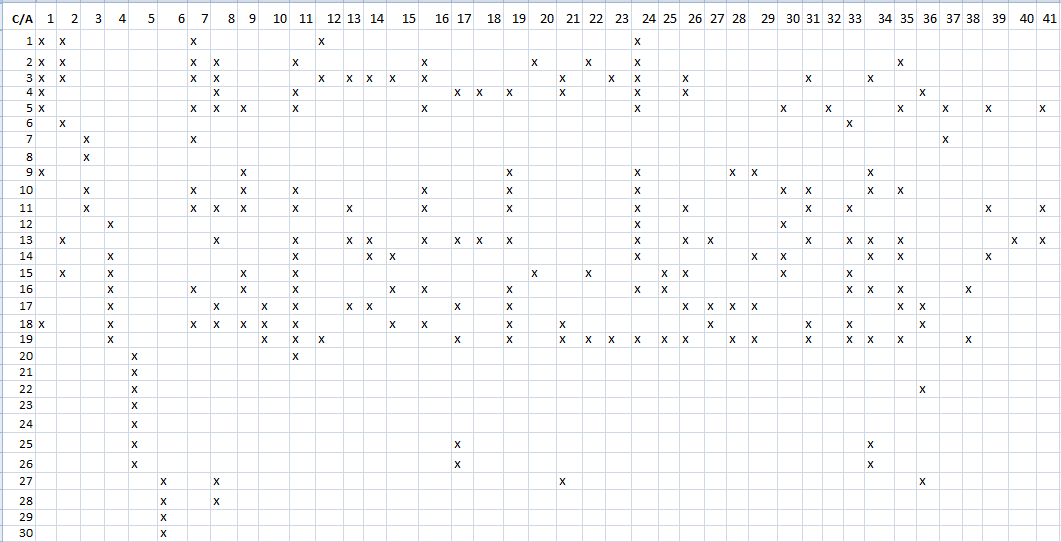
\includegraphics[keepaspectratio=true,scale=0.9]{figuras/Figura_1.png}
\caption{Rastreabilidade de Características para CMSs populares Parte 1}
\label{Rastreabuilidade_Popular_1}
\end{figure}
\end{landscape}

\begin{landscape}
\begin{figure}[h]
\centering
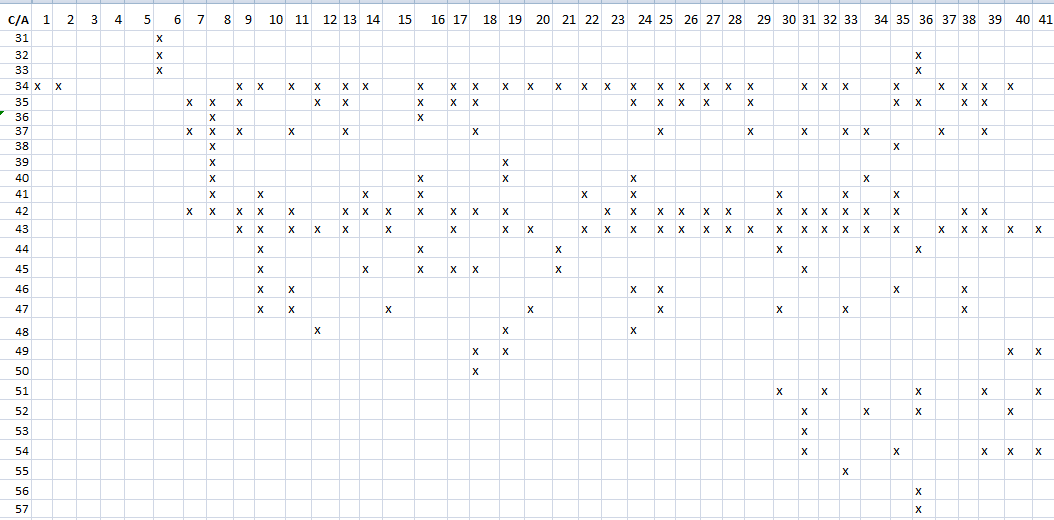
\includegraphics[keepaspectratio=true,scale=0.9]{figuras/Figura_2.png}
\caption{Rastreabilidade de Características para CMSs populares Parte 2}
\label{Rastreabuilidade_Popular_2}
\end{figure}
\end{landscape}


\begin{figure}[h]
\centering
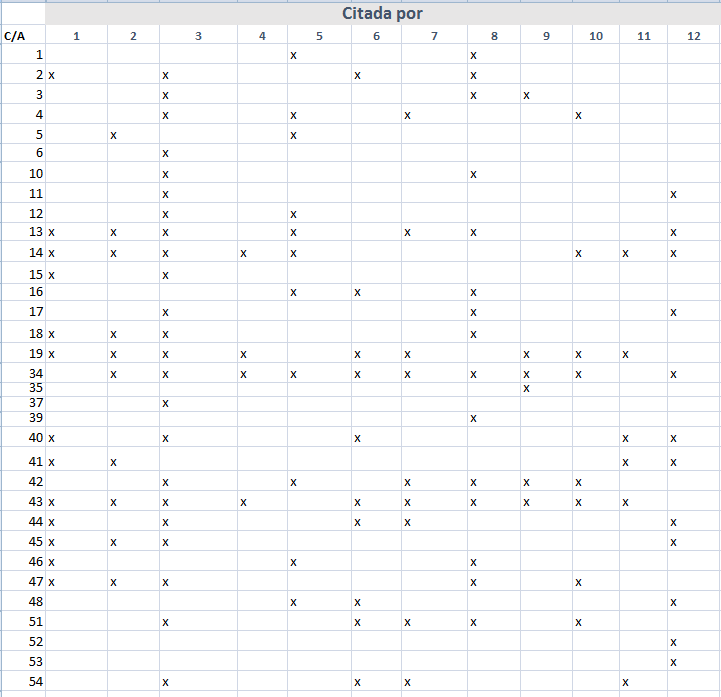
\includegraphics[keepaspectratio=true,scale=0.70]{figuras/Figura_3.png}
\caption{Rastreabilidade de Características para CMSs não populares Parte 1}
\label{Rastreabuilidade_Não_Popular_3}
\end{figure}



\begin{figure}[h]
\centering
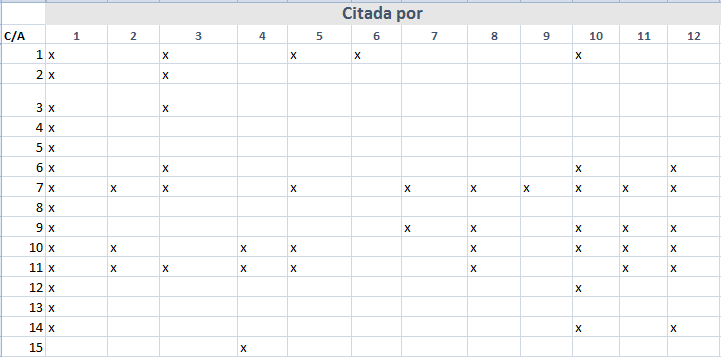
\includegraphics[keepaspectratio=true,scale=0.65]{figuras/Figura_4.png}
\caption{Rastreabilidade de Características para CMSs não populares Parte 2}
\label{Rastreabuilidade_Não_Popular_4}
\end{figure}

A figura \ref{Rastreabuilidade_Não_Popular_4} mostra somente o mapeamento para as novas características.

\chapter{Questionários}
\label{Questionários}

\section{Questionário 1 - Levantamento de Características de CMSs}
\label{Quest1}

Este formulário faz parte de um trabalho de conclusão de curso, cujo objetivo é identificar características importantes de Sistemas gerenciadores de conteúdo para servirem de apoio a quem vai escolher um determinado produto de CMS para ser usado no desenvolvimento de um site WEB. 
Ele se baseia em características pesquisadas na literatura como sendo importantes para produtos de CMS. Ao responder as próximas questões use as definições a seguir:

Adequação Funcional: É o grau com que o produto provê funções que atendem as necessidades explícitas e implícitas quando usado sobre condições específicas.

Performance: Desempenho relativo à quantidade de recursos usados sobre condições específicas.

Compatibilidade: É o grau com que o produto pode trocar informações com outros produtos e/ou realizar suas funções, enquanto compartilha o mesmo ambiente de hardware e software.

Usabilidade: É o grau com que o produto pode atingir os objetivos específicos de usuários específicos com eficácia, eficiência e satisfação, em um determinado contexto de uso.

Confiabilidade: É o grau com que o produto realiza determinadas funções, sobre condições específicas em um tempo específico.

Segurança: É o grau com que o produto protege dados e informações, de modo que exista graus de acesso a determinadas partes do produto, para determinados tipos e níveis de autorização.

Manutenibilidade: É o grau de eficácia e eficiência com que o produto pode ser modificado pelos seus respectivos mantenedores.

Portabilidade: É o grau com que o produto pode ser transferido de um ambiente de uso para o outro.

Eficácia em uso : Acurácia e completude com que os usuários conseguem atingir seus objetivos.

Eficiência em uso: Recursos gastos em relação a acurácia e completude com que os usuários atingem seus objetivos.

Satisfação do cliente: É o grau com que as necessidades do usuário são satisfeitas pelo uso do produto em um contexto específico.

Inexistência de Risco: É o grau com que o produto mitiga os riscos econômicos, os riscos a vida humana, a saúde, e ao ambiente.

Completude: grau o qual um produto ou sistema pode ser utilizado com eficácia, eficiência,  liberdade de riscos, satisfação em todos os contextos de utilização especificados.

\textbf{1) No momento de escolher um determinado CMS para uma aplicação você leva em conta o Licenciamento?}*

()Sim
                             
()Não

\textbf{2) Você prefere um CMS software Livre ou software proprietário para desenvolver suas aplicações?}* 

() Software Livre

() Software Proprietário

\textbf{2.1) Justifique sua resposta:}

\textbf{3) No que diz respeito à características funcionais do CMS, quais delas você julga como importantes ou indispensáveis em um CMS? *}

\textit{Escolha quantas forem necessárias e utilize o campo "Outros" para indicar o que achar importante que esteja faltando na lista (no caso de mais de uma opção separe-as com virgula).}

() Facilidade de interação do CMS com várias ferramentas. (ex: outras linguagens, bancos de dados, frameworks de programação, etc)
  
() Capacidade de armazenar dados em bancos de dados relacionais.
 
() Boa capacidade para realizar pesquisas ou buscas de conteúdos no próprio site.
 
() Permitir upload de uma grande quantidade de tipos de arquivos Exemplos: (Word, Excel, RTF, PDF, etc).
 
() Permitir download de uma grande quantidade de tipos de arquivos Exemplos: (Word, Excel, RTF, PDF, etc).
 
() Suporte para conteúdos multimídia (ex: vídeos, músicas, etc).
 
() Habilidade para controlar e gerenciar múltiplas versões do mesmo conteúdo.
 
() Geração automática de Interface de Usuário.
 
() Permitir gerenciamento de usuários.
 
() Permitir gerenciamento de arquivos.
 
() Capacidade de executar Backup dos conteúdos do site.
 
() Suporte a Fóruns de discussão.
 
() Suporte a comentários.
 
() Outro: 
 
\textbf{4) A quantidade de templates ou plugins disponíveis para um determinado CMS é um fator importante para escolha desse CMS? *}

()Sim

()Não


\textbf{5) No que diz respeito a Usabilidade, quais características você julga como importantes ou indispensáveis na hora de escolher um CMS? *}

\textit{Escolha quantas características opções forem necessárias e, caso existam características não presentes na lista, inclua-as no campo "outro" separadas por vírgula.}

()  Interatividade alta.

() Facilidade em criar novos conteúdos.

() Fácil utilização

() Disponibilidade de documentação de fácil uso e entendimento

() Outro: 


\textbf{6) No que diz respeito a Portabilidade, quais características você julga como importante ou indispensáveis na hora de se escolher um CMS para sua aplicação? *}

\textit{Escolha quantas características opções forem necessárias e, caso existam características não presentes na lista, inclua-as no campo "outro" separadas por vírgula.}

()  Permitir o gerenciamento de conteúdo em qualquer navegador( Até os de celular)

() Ser multiplataforma (Funcionar independente de sistema operacional) .

() Ser fácil de instalar.

() Outro: 


\textbf{7) No que diz respeito a Manutenibilidade, quais características você julga como importante ou indispensáveis na hora de se escolher um CMS para sua aplicação? *}

\textit{Escolha quantas características opções forem necessárias e, caso existam características não presentes na lista, inclua-as no campo "outro" separadas por vírgula.}

() Fácil configuração para interagir com outros sites.

() Modularidade.

() Boa Taxonomia

() Facilidade em Manutenção.

() Modificabilidade

() Liberdade para alteração de um template específico.

() Reusabilidade

() Outro: 


\textbf{8) No que diz respeito a Segurança, quais características você julga como importante ou indispensáveis na hora de se escolher um CMS para sua aplicação? *}

\textit{Escolha quantas características opções forem necessárias e, caso existam características não presentes na lista, inclua-as no campo "outro" separadas por vírgula.}

() Permitir a restrição de  acesso de a um determinado usuário a funcionalidades, de acordo com o seu perfil de acesso.
  
() Proteção contra SQL injection

() Mecanismo anti phishing

() Mecanismo anti plágio.

() Outro:
 
\textbf{9) No que diz respeito à Performance (desempenho) quais características no seu entender que podem prejudicar o desempenho do site na hora de se escolher um CMS para sua aplicação? *}

\textit{Escolha quantas características opções forem necessárias e, caso existam características não presentes na lista, inclua-as no campo "outro" separadas por vírgula.}

 () Tempo de carregamento da página.
 
 ()Total de Requisições feitas pela página ao se disparar uma determinada ação (funcionalidade, tarefa, atividade, etc).
 
 ()Tamanho de Página em KB.
 
() Outro: 

\textbf{10) A popularidade influencia você a escolher um determinado CMS ? *
}

()  Sim
  
() Não
 
\textbf{10.1) Justifique sua resposta. *}
 
\textbf{11) A arquitetura de um CMS é um fator preponderante para a sua escolha ? *}
 () Sim
 
() Não
 
\textbf{11.1) Justifique a sua resposta *}
 
\textbf{12) O tamanho da comunidade de pessoas que usam o CMS é um fator preponderante para a escolha de um determinado CMS? *}

()  Sim
  
() Não
 
12.1) Justifique sua resposta
 
\textbf{13) Qua(l)is das características abaixo você julga também importante ter em um CMS, além das já perguntadas? *}

\textit{Para responder essa questão corretamente veja as definições no topo da página}

()  Compatibilidade

() Confiabilidade

() Eficácia em uso

() Satisfação do Cliente

() Inexistência de Riscos

() Flexibilidade

() Completude

() Eficiência em uso

() Nenhuma dessas, pois depende da aplicação
 
\textbf{14) Além de todas as características apresentadas você gostaria de acrescentar outra que fosse importante para um CMS?}

Justifique sua resposta.

\textbf{\textit{*Pergunta Obrigatória}}
 
 
\section{Questionário 2 - Validação do Método Proposto }
\label{Questionário_2}

Validação de método para a seleção de sistemas CMS.
Questionário desenvolvido por Thiago S. Honorato, estudante de graduação da Engenharia de Software da Universidade de Brasília (UnB) para a finalidade de validar um método proposto para o auxílio da seleção de sistemas CMS. O questionário se baseia num conjunto de métricas levantadas da ISO 25000, mapeadas de acordo com as características de CMS da literatura. Características validadas por meio de um questionário aplicado anteriormente em comunidades de Sistemas CMS no facebook.
O questionário faz parte de um trabalho de conclusão de curso submetido pela Universidade de Brasília.


Para responder o questionário considere as escalas na descrição de cada pergunta e responda de acordo com as afirmativas.

Grato a Compreensão. 



\textit{\textbf{*Obrigatório}}

\textbf{1) No que diz respeito a Adequação Funcional complete: a completude funcional de um determinado CMS é -------. *}

\textit{Considere como completude funcional o conjunto de funcionalidades necessárias para satisfazer os objetivos da sua aplicação. Considere que: 1 - Sem Importância, 2 - Pouco Importante, 3 - Muito Importante, 4 - Extremamente Importante}

()1
()2
()3
()4




\textbf{2) No que diz respeito a Usabilidade complete: as mensagens exibidas pelo CMS são ---------. *}

\textit{Considere como mensagem: mensagens de ajuda, textos informativos e demais textos presentes na página que influenciam tomadas de decisão. Considere que: 1 - Sem Importância, 2 - Pouco Importante, 3 - Muito Importante, 4 - Extremamente Importante}

()1
()2
()3
()4




\textbf{3) No que diz respeito a Usabilidade complete :É ----------- a documentação disponível auxíliar no aprendizado do CMS. *}

\textit{Considere que: 1 - Sem Importância, 2 - Pouco Importante, 3 - Muito Importante, 4 - Extremamente Importante}

()1
()2
()3
()4




\textbf{4) No que diz respeito a Usabilidade complete: o layout é ----------- em um determinado CMS. *}

\textit{Considere que: 1 - Sem Importância, 2 - Pouco Importante, 3 - Muito Importante, 4 - Extremamente Importante}

()1
()2
()3
()4




\textbf{5) No que diz respeito a Segurança complete: o controle de acesso é --------- em um determinado CMS. *}

\textit{Considere que: 1 - Sem Importância, 2 - Pouco Importante, 3 - Muito Importante, 4 - Extremamente Importante}

()1
()2
()3
()4




\textbf{6) No que diz respeito a Segurança, complete: evitar que dados sejam corrompidos em um site feito com CMS é ----------- *}

\textit{Considere que: 1 - Sem Importância, 2 - Pouco Importante, 3 - Muito Importante, 4 - Extremamente Importante}

()1
()2
()3
()4




\textbf{7) No que diz respeito a Portabilidade complete: adaptar o CMS a um determinado ambiente operacional é ---------- *}

\textit{Considere que: 1 - Sem Importância, 2 - Pouco Importante, 3 - Muito Importante, 4 - Extremamente Importante}

()1
()2
()3
()4




\textbf{8) No que diz respeito a Manutenabilidade complete: modificar um CMS para resolver um determinado problema é -------- *}

\textit{Considere que: 1 - Sem Importância, 2 - Pouco Importante, 3 - Muito Importante, 4 - Extremamente Importante}

()1
()2
()3
()4




\textbf{9) No que diz respeito a Manutenabilidade complete. É ------------- o CMS possuir módulos reusáveis. *}

\textit{Considere que: 1 - Sem Importância, 2 - Pouco Importante, 3 - Muito Importante, 4 - Extremamente Importante}

()1
()2
()3
()4




\textbf{10) No que diz respeito a Manutenabilidade complete: o relacionamento entre os componentes é ------------ para o funcionamento do módulo. *}

Considere que: 1 - Sem Importância, 2 - Pouco Importante, 3 \textit{- Muito Importante, 4 - Extremamente Importante}

1
2
3
4




\textbf{11) No que diz respeito a Manutenabilidade complete : testes de sistema são ----------------- para um CMS. *}

\textit{Considere que: 1 - Sem Importância, 2 - Pouco Importante, 3 - Muito Importante, 4 - Extremamente Importante}

()1
()2
()3
()4




\textbf{12) No que diz respeito a Performance complete : a quantidade de tarefas que pode ser realizada por período de tempo é -------------. *}

\textit{Considere que: 1 - Sem Importância, 2 - Pouco Importante, 3 - Muito Importante, 4 - Extremamente Importante}

()1
()2
()3
()4




\textbf{13) No que diz respeito a Performance complete: a utilização de memória e outros recursos de hardware é -------- em um CMS. *}

\textit{Considere que: 1 - Sem Importância, 2 - Pouco Importante, 3 - Muito Importante, 4 - Extremamente Importante}

()1
()2
()3
()4




\textbf{14) No que diz respeito a confiabilidade complete: a capacidade de falhas serem identificadas e corrigidas em um projeto com uso de CMS é -----------. *}

\textit{Considere que: 1 - Sem Importância, 2 - Pouco Importante, 3 - Muito Importante, 4 - Extremamente Importante}

()1
()2
()3
()4




\textbf{15) No que diz respeito a Confiabilidade complete: um site que utiliza CMS prover disponibilidade 24/7 é ------------. *}

\textit{Considere 24/7 como 24 horas os 7 dias da semana .Considere que: 1 - Sem Importância, 2 - Pouco Importante, 3 - Muito Importante, 4 - Extremamente Importante}

()1
()2
()3
()4




\textbf{16) No que diz respeito a Confiabilidade complete: ------------ o CMS ser tolerante a falhas. *}

\textit{Considere como tolerância a falhas a capacidade do CMS de operar conforme o esperado, porém estando sujeito a falhas de hardware/e ou software. Considere que: 1 - Sem Importância, 2 - Pouco Importante, 3 - Muito Importante, 4 - Extremamente Importante}

()1
()2
()3
()4




\textbf{17) No que diz respeito a Confiabilidade complete: é ---------------- o CMS se recuperar após uma falha. *}

\textit{Considere que: 1 - Sem Importância, 2 - Pouco Importante, 3 - Muito Importante, 4 - Extremamente Importante}

()1
()2
()3
()4


\textbf{18) No que diz respeito a Efetividade complete: é ----------- um usuário realizar suas atividades e conseguir completa-las de forma correta. *}

\textit{Considere que: 1 - Sem Importância, 2 - Pouco Importante, 3 - Muito Importante, 4 - Extremamente Importante}

()1
()2
()3
()4


\textbf{19) No que diz respeito a Cobertura do Contexto em uso complete: a flexibilidade em uso de determinado CMS é {-----------------}. *}

\textit{Considere que: 1 - Sem Importância, 2 - Pouco Importante, 3 - Muito Importante, 4 - Extremamente Importante}

()1
()2
()3
()4


\chapter{GQM - Métricas Definidas}
\label{GQM-Métricas-Apendice}

OBS: Os valores descritos para a interpretação das métricas são sugestões. Para uma análise mais precisa de valores é necessária uma investigação mais profunda, seja na literatura, ou por meio de experimentação. A \citeonline{iso_25023} não cita esses valores na descrição de suas métricas. 


\section{Métricas - Adequação Funcional}
\label{AdequaçãoFuncional}


\begin{longtable}{|p{115pt}|p{265pt}|}
 	\caption{M1 - Cobertura Funcional - Adaptado de \citeonline{iso_25023}} 
 	\label{M001}\\
 	\hline
 	 	 {\raggedright \textbf{Questão}}
 	 	 & {\raggedright {01}}\\
 	\hline
 	 {\raggedright \textbf{ID}}
 	 & {\raggedright {AF-CF-M001}}\\
 	
 	\hline
 		{\raggedright \textbf{Nome}}
 	 	 & {\raggedright Cobertura Funcional}
 	 	 \\\hline
 	 {\raggedright \textbf{Característica}}
 	 & {\raggedright   Adequação Funcional }\\	
 	\hline
 	 {\raggedright \textbf{SubCaracterística}}
 	 & {\raggedright Completude Funcional} 	
 \\	\hline
 	 {\raggedright \textbf{Descrição 
 	 \\(Questão)}} 
 	 & {\raggedright  Qual percentual (\%) de adequação funcional possui o software?} \\

 	\hline
 	 {\raggedright \textbf{Função de Medição \\ (fórmula)}}
 	 & {\raggedright {\tiny{A = Numero de perguntas que obtiverem resposta sim.
 	\\B = Total de perguntas do questionário.
 	\\ X = (A/B) * 100 \%}}} 
 	\\\hline
 	{\raggedright \textbf{Método \\(Forma de coleta)}}
 	 & {\raggedright \tiny{1. Aplicar questionário.
 	                  \\ 2.	Calcular o valor A. \\
 	                 3.	Aplicar a fórmula.
 	                 \\}
  	                }\\\hline
 	{\raggedright \textbf{Interpretação}}
 	 & {\raggedright 
 	                 Quanto maior melhor.
 	                 \\\tiny{0 < x <= 29 é pessimo
 	                 \\30 < x <= 49 é regular
 	                 \\50 < x <= 70 é bom
 	                 \\71 <= x <= 100 é excelente}
 	                 \\
 	  }\\
 
 	\hline
\end{longtable}

\section{Métricas - Usabilidade}
\label{Usabilidade}

\begin{longtable}{|p{115pt}|p{265pt}|}
 	\caption{M2 - Percentual de mensagens claras - Adaptado de \citeonline{iso_25023}} 
 	\label{M002}\\
 	\hline
 	{\raggedright \textbf{Questão}}
 	 	 	 & {\raggedright {02}}\\
 	 	\hline
 	 {\raggedright \textbf{ID}}
 	 & {\raggedright {UB-OP-M001}}\\	
 	\hline
 		{\raggedright \textbf{Nome}}
 	 	 & {\raggedright Percentual de mensagens claras}\\	 	
 	 	\hline
 	 {\raggedright \textbf{Característica}}
 	 & {\raggedright  Usabilidade }\\
 	
 	\hline
 	 {\raggedright \textbf{SubCaracterística}}
 	 & {\raggedright Operacionalidade} 	
 \\	\hline
 	 {\raggedright \textbf{Descrição 
 	 \\(Questão)}} 
 	 & {\raggedright  Qual percentual (\%) de  mensagens exibidas pelo sistema  que podem ser facilmente entendidas?} \\
	\hline
 	 {\raggedright \textbf{Função de Medição \\ (fórmula)}}
 	 & {\raggedright {\tiny{A = Soma de todas as notas das mensagens.\\
 	 B = Número total de mensagens avaliadas.\\
 	 X= (A/B)*100\%.}}} 
 	\\\hline
 	{\raggedright \textbf{Método \\(Forma de coleta)}}
 	 & {\raggedright \tiny{1.Identificar um conjunto de mensagens no sistema.\\
 	 2.	Elaborar um questionário para validar semanticamente as mensagens.\\
 	 3.	Calcular nota de todas as mensagens válidas.\\
 	 4.	Somar todas as notas de todas as mensagens.\\
 	 5.	Calcular o percentual.}
  	                }\\\hline
 	{\raggedright \textbf{Interpretação}}
 	 & {\raggedright \tiny{Quanto maior melhor.\\
 	                 0 < x <= 29 é péssimo\\
 	                 30 < x <= 49 é regular\\
 	                 50 < x <= 70 é bom\\
 	                 71 <= x <= 100 é excelente}
 	  }\\
 
 	\hline
 	 
\end{longtable}

\begin{longtable}{|p{115pt}|p{265pt}|}
 	\caption{M3 - Documentação Plena - Adaptado de \citeonline{iso_25023}} 
 	\label{M003}\\
 	\hline
 	{\raggedright \textbf{Questão}}
 	 	 	 & {\raggedright {03}}\\
 	 	\hline
 	 {\raggedright \textbf{ID}}
 	 & {\raggedright {UB-AP-M001}}\\	
 	\hline
 		{\raggedright \textbf{Nome}}
 	 	 & {\raggedright Documentação plena}\\	 	
 	 	\hline
 	 {\raggedright \textbf{Característica}}
 	 & {\raggedright  Usabilidade }\\
 	
 	\hline
 	 {\raggedright \textbf{SubCaracterística}}
 	 & {\raggedright Aprendizado} 	
 \\	\hline
 	 {\raggedright \textbf{Descrição 
 	 \\(Questão)}} 
 	 & {\raggedright Qual a proporção de funcionalidades descritas na documentação que podem ajudar ou facilitar o uso do software?} \\
	\hline
 	 {\raggedright \textbf{Função de Medição \\ (fórmula)}}
 	 & {\raggedright {\tiny{A = Número de funcionalidades descritas na documentação.\\
 	 B =  Número total de funcionalidades implementadas.\\
 	 X= (A/B)*100 \%}}} 
 	\\\hline
 	{\raggedright \textbf{Método \\(Forma de coleta)}}
 	 & {\raggedright \tiny{1.Logar com o perfil de Admin (Possui todas as funcionalidades).\\
 	 2.	Anotar e contar todas as funcionalidades observadas.\\
 	 3.	Verificar na documentação se as funcionalidades que são descritas.\\
 	 4.	Contar a quantidade de funcionalidades descritas.\\
 	 5.	Fazer calculo da proporção utilizando a fórmula.
 	 }
  	                }\\\hline
 	{\raggedright \textbf{Interpretação}}
 	 & {\raggedright \tiny{Quanto maior melhor.\\
 	 0 < X <= 25\% é péssimo\\
 	 25\% < X <= 50\% é regular\\
 	 50\% < X <=75\% é bom\\
 	 75\% < X <= 100\% é excelente.}
 	  }\\
 
 	\hline
 	 
\end{longtable}
\clearpage
\begin{longtable}{|p{115pt}|p{265pt}|}
 	\caption{M4 - Percentual de elementos personalizáveis - Adaptado de \citeonline{iso_25023}} 
 	\label{M008}\\
 	\hline
 	{\raggedright \textbf{Questão}}
 	 	 	 & {\raggedright {04}}\\
 	 	\hline
 	 {\raggedright \textbf{ID}}
 	 & {\raggedright {US–EST–M001}}\\	
 	\hline
 		{\raggedright \textbf{Nome}}
 	 	 & {\raggedright Percentual de elementos personalizáveis}\\	 	
 	 	\hline
 	 {\raggedright \textbf{Característica}}
 	 & {\raggedright  Usabilidade }\\
 	
 	\hline
 	 {\raggedright \textbf{SubCaracterística}}
 	 & {\raggedright Estética} 	
 \\	\hline
 	 {\raggedright \textbf{Descrição 
 	 \\(Questão)}} 
 	 & {\raggedright  Qual percentual (\%) de elementos de interface que podem ser personalizados?} \\
	\hline
 	 {\raggedright \textbf{Função de Medição \\ (fórmula)}}
 	 & {\raggedright {\tiny{A = Número de elementos de interface que podem ser personalizados.\\
 	 B = número total de elementos de interface.\\ 
 	 X = (A/B) * 100 \%}}} 
 	\\\hline
 	{\raggedright \textbf{Método \\(Forma de coleta)}}
 	 & {\raggedright \tiny{1.Escolher uma tela do sistema.\\
 	 2.	Contar o número de elementos da tela escolhida.\\
 	 3.	Contar o número de elementos personalizáveis.\\
 	 4.	Aplicar fórmula.}
  	                }\\\hline
 	{\raggedright \textbf{Interpretação}}
 	 & {\raggedright \tiny{Quanto maior melhor.\\
 	  	 0 < X <= 25\% é péssimo\\
 	  	 25\% < X <= 50\% é regular\\
 	  	 50\% < X <=75\% é bom\\
 	  	 75\% < X <= 100\% é excelente.}
 	  }\\
 
 	\hline
 	 
\end{longtable}

\section{Métricas - Segurança}
\begin{longtable}{|p{115pt}|p{265pt}|}
 	\caption{M5 - Controle de acesso - Adaptado de \citeonline{iso_25023}} 
 	\label{M004}\\
 	\hline
 	{\raggedright \textbf{Questão}}
 	 	 	 & {\raggedright {10}}\\
 	 	\hline
 	 {\raggedright \textbf{ID}}
 	 & {\raggedright {SE-CO-M001}}\\	
 	\hline
 		{\raggedright \textbf{Nome}}
 	 	 & {\raggedright Controle de acesso}\\	 	
 	 	\hline
 	 {\raggedright \textbf{Característica}}
 	 & {\raggedright  Segurança }\\
 	
 	\hline
 	 {\raggedright \textbf{SubCaracterística}}
 	 & {\raggedright Confidencialidade} 	
 \\	\hline
 	 {\raggedright \textbf{Descrição 
 	 \\(Questão)}} 
 	 & {\raggedright  O quão controlável é o acesso ao sistema?} \\
	\hline
 	 {\raggedright \textbf{Função de Medição \\ (fórmula)}}
 	 & {\raggedright {\tiny{A = Número de operações/atividades exclusivas do perfil Autor que foi acessada pelo perfil Assinante.\\
 	 B = Número de tentativas de acesso a operação/atividade exclusiva realizadas.\\
 	 X = A/B}}} 
 	\\\hline
 	{\raggedright \textbf{Método \\(Forma de coleta)}}
 	 & {\raggedright \tiny{1.Criar na aplicação dois usuários distintos. Um usuário comum e um usuário administrador.\\
 	 2.	Dar permissões exclusivas para o usuário administrador.\\
 	 3.	Logar na aplicação como usuário comum e tentar um acesso que só  o usuário administrador consiga realizar.\\
 	 4.	Observar se o sistema permite ou não acesso.}}\\\hline
 	{\raggedright \textbf{Interpretação}}
 	 & {\raggedright \tiny{Quanto mais próximo de 0 melhor.\\
 	 X > 2 é péssimo\\
 	 1 < X <= 2 é regular\\
 	 0 < X <= 1 é bom\\
 	 X = 0 é excelente}}\\
 
 	\hline
 	 
\end{longtable}


\begin{longtable}{|p{115pt}|p{265pt}|}
 	\caption{M6 - Prevenção a dados corrompidos - Adaptado de \citeonline{iso_25023}} 
 	\label{M011}\\
 	\hline
 	{\raggedright \textbf{Questão}}
 	 	 	 & {\raggedright {11}}\\
 	 	\hline
 	 {\raggedright \textbf{ID}}
 	 & {\raggedright {SEG–INT–M001}}\\	
 	\hline
 		{\raggedright \textbf{Nome}}
 	 	 & {\raggedright Prevenção a dados corrompidos.}\\	 	
 	 	\hline
 	 {\raggedright \textbf{Característica}}
 	 & {\raggedright  Segurança }\\
 	
 	\hline
 	 {\raggedright \textbf{SubCaracterística}}
 	 & {\raggedright Integridade} 	
 \\	\hline
 	 {\raggedright \textbf{Descrição 
 	 \\(Questão)}} 
 	 & {\raggedright  Dados corrompidos podem ser evitados?} \\
	\hline
 	 {\raggedright \textbf{Função de Medição \\ (fórmula)}}
 	 & {\raggedright {\tiny{A = Número de casos de dados corrompidos que ocorreram ao se executar uma determinada tarefa, ou conjunto de tarefas.\\
 	 B = Número de casos de dados corrompidos previstos.\\ 
 	 X = (A/B) }}} 
 	\\\hline
 	{\raggedright \textbf{Método \\(Forma de coleta)}}
 	 & {\raggedright \tiny{1. Escolher um conjunto de tarefas em que podem haver dados corrompidos.\\
 	 2.	Contar o número de situações em que podem acontecer dados corrompidos ao se executar as tarefas propostas.\\
 	 3.	Executar as tarefas propostas.\\
 	 4.	Contar o número de situações em que de fato ocorreram dados corrompidos.}}\\\hline
 	{\raggedright \textbf{Interpretação}}
 	 & {\raggedright \tiny{Quanto menor melhor.\\
 	  	  X > 3 é péssimo\\
 	  	 2 < X < 3\ é regular\\
 	  	 1 <= X <= 2\% é bom\\
 	  	 X = 0 é excelente.}
 	  }\\
 
 	\hline
 	 
\end{longtable}

\section{Métricas - Portabilidade}

\begin{longtable}{|p{115pt}|p{265pt}|}
 	\caption{M7 - Mudança de configuração - Adaptado de \cite{9126-2}} 
 	\label{M005}\\
 	\hline
 	{\raggedright \textbf{Questão}}
 	 	 	 & {\raggedright {05}}\\
 	 	\hline
 	 {\raggedright \textbf{ID}}
 	 & {\raggedright {POR-AD-M001}}\\	
 	\hline
 		{\raggedright \textbf{Nome}}
 	 	 & {\raggedright Mudança de configuração}\\	 	
 	 	\hline
 	 {\raggedright \textbf{Característica}}
 	 & {\raggedright  Portabilidade }\\
 	
 	\hline
 	 {\raggedright \textbf{SubCaracterística}}
 	 & {\raggedright Adaptabilidade} 	
 \\	\hline
 	 {\raggedright \textbf{Descrição 
 	 \\(Questão)}} 
 	 & {\raggedright  O usuário ou mantenedor pode adaptar o  software ao ambiente?} \\
	\hline
 	 {\raggedright \textbf{Função de Medição \\ (fórmula)}}
 	 & {\raggedright {\tiny{T = Soma do tempo de operação gasto pelo usuário para completar a adaptação do software ao ambiente do usuário, quando ele tentar instalá-lo ou modificar sua configuração.
 	 X = T.
 	 }}} 
 	\\\hline
 	{\raggedright \textbf{Método \\(Forma de coleta)}}
 	 & {\raggedright \tiny {1.Selecionar 4 plugins e 1 tema a serem instalados na ferramenta.\\
 	 2.	Realizar três medições do processo de customização da ferramenta com os plugins e temas.\\
 	 3.	Calcular média aritmética das três medições realizadas.}}\\
 	 \hline
 	{\raggedright \textbf{Interpretação}}
 	 & {\raggedright \tiny{Quanto mais próximo de 0 melhor (mm:ss).\\
 	 X > 15:00 é péssimo\\
 	 10:00 < X <= 15:00 é regular\\
 	 05:00 < X <= 10:00 é bom\\
 	 X <= 05:00 é excelente}
 	  }\\
 
 	\hline
 	 
\end{longtable}

\section{Métricas - Manutenibilidade}

\begin{longtable}{|p{115pt}|p{265pt}|}
 	\caption{M8 - Complexidade de modificação - Adaptado de \citeonline{iso_25023}} 
 	\label{M006}\\
 	\hline
 	{\raggedright \textbf{Questão}}
 	 	 	 & {\raggedright {08}}\\
 	 	\hline
 	 {\raggedright \textbf{ID}}
 	 & {\raggedright {MAN-MOF-M001}}\\	
 	\hline
 		{\raggedright \textbf{Nome}}
 	 	 & {\raggedright Complexidade de modificação}\\	 	
 	 	\hline
 	 {\raggedright \textbf{Característica}}
 	 & {\raggedright  Manutenabilidade }\\
 	
 	\hline
 	 {\raggedright \textbf{SubCaracterística}}
 	 & {\raggedright Modificabilidade} 	
 \\	\hline
 	 {\raggedright \textbf{Descrição 
 	 \\(Questão)}} 
 	 & {\raggedright  O mantenedor pode modificar o software para resolver um problema?} \\
	\hline
 	 {\raggedright \textbf{Função de Medição \\ (fórmula)}}
 	 & {\raggedright {\tiny{A = Tempo gasto para modificar.
 	 B = Número de \textit{issues} feitas.
 	 X = A/B
 	 }}} 
 	\\\hline
 	{\raggedright \textbf{Método \\(Forma de coleta)}}
 	 & {\raggedright \tiny{1.	Escolher um período de tempo específico (hora, mês, dia, semana).\\
 	 2.	Identificar a quantidade de mudanças feitas na aplicação nesse período de tempo escolhido. (Observar o repositório)\\
 	 3.	Levantar a quantidade de mudanças identificadas no periodo de tempo proposto.\\
 	 }
  	                }\\\hline
 	{\raggedright \textbf{Interpretação}}
 	 & {\raggedright \tiny{Quanto menor melhor.\\
 	                 0 < x <= 3 é excelente\\
 	                 3 < x <= 5 é bom\\
 	                 5 < x <= 10 é ruim\\
 	                 >10 é péssimo}
 	  }\\
 
 	\hline
 	 
\end{longtable}

\begin{longtable}{|p{115pt}|p{265pt}|}
 	\caption{M9 - Condensabilidade - Adaptado de \citeonline{iso_25023}} 
 	\label{M007}\\
 	\hline
 	{\raggedright \textbf{Questão}}
 	 	 	 & {\raggedright {06}}\\
 	 	\hline
 	 {\raggedright \textbf{ID}}
 	 & {\raggedright {MAN-MODU-M001}}\\	
 	\hline
 		{\raggedright \textbf{Nome}}
 	 	 & {\raggedright Condensabilidade}\\	 	
 	 	\hline
 	 {\raggedright \textbf{Característica}}
 	 & {\raggedright  Manutenabilidade}\\
 	
 	\hline
 	 {\raggedright \textbf{SubCaracterística}}
 	 & {\raggedright Modularidade} 	
 \\	\hline
 	 {\raggedright \textbf{Descrição 
 	 \\(Questão)}} 
 	 & {\raggedright  
 	 Qual é a relação entre os componentes presentes em um determinado modulo de um software? } \\
	\hline
 	 {\raggedright \textbf{Função de Medição \\ (fórmula)}}
 	 & {\raggedright {\tiny	A = Número de componentes que quando sofrem mudanças não afetam outros componentes.\\
 	 B = Número total de componentes do módulo em questão.\\
 	 X = A/B.}}
 	\\\hline
 	{\raggedright \textbf{Método \\(Forma de coleta)}}
 	 & {\raggedright \tiny{1.Identificar um modulo no sistema.\\
 	 2.	Identificar o total de componentes.\\
 	 3.	Identificar quais componentes quando alterados impactam outros componentes.\\
 	 4.	Calcular o resultado.\\}
  	                }\\\hline
 	{\raggedright \textbf{Interpretação}}
 	 & {\raggedright \tiny{Quanto mais próximo de 1 melhor.\\
 	                 0 < x <= 0,29 é péssimo\\
 	                 0,30 < x <= 0,59 é regular\\
 	                 0,6 < x <= 0,89 é bom\\
 	                 0,9 <= x = 1 é excelente}
 	  }\\
 
 	\hline

 	 
\end{longtable}



\begin{longtable}{|p{115pt}|p{265pt}|}
 	\caption{M10 - Percentual de módulos reusáveis - Adaptado de \citeonline{iso_25023}} 
 	\label{M009}\\
 	\hline
 	{\raggedright \textbf{Questão}}
 	 	 	 & {\raggedright {07}}\\
 	 	\hline
 	 {\raggedright \textbf{ID}}
 	 & {\raggedright {MAN– REU–M001}}\\	
 	\hline
 		{\raggedright \textbf{Nome}}
 	 	 & {\raggedright Percentual de módulos reusáveis}\\	 	
 	 	\hline
 	 {\raggedright \textbf{Característica}}
 	 & {\raggedright  Manutenibilidade }\\
 	
 	\hline
 	 {\raggedright \textbf{SubCaracterística}}
 	 & {\raggedright Reusabilidade} 	
 \\	\hline
 	 {\raggedright \textbf{Descrição 
 	 \\(Questão)}} 
 	 & {\raggedright  Qual percentual (\%) de módulos do sistema que podem ser reutilizados?} \\
	\hline
 	 {\raggedright \textbf{Função de Medição \\ (fórmula)}}
 	 & {\raggedright {\tiny{A = Número de módulos do sistema que podem ser reutilizados.\\
 	 B = número total de modulos do sistema.\\ 
 	 X = (A/B) * 100 \%}}} 
 	\\\hline
 	{\raggedright \textbf{Método \\(Forma de coleta)}}
 	 & {\raggedright \tiny {1.Identificar o número de módulos do sistema.\\
 	 2.	Contar o número de módulos do sistema que podem ser reutilizados.\\
 	 3.	Aplicar fórmula.}
  	                }\\\hline
 	{\raggedright \textbf{Interpretação}}
 	 & {\raggedright \tiny{Quanto maior melhor.\\
 	  	 0 < X <= 25\% é péssimo\\
 	  	 25\% < X <= 50\% é regular\\
 	  	 50\% < X <=75\% é bom\\
 	  	 75\% < X <= 100\% é excelente.}
 	  }\\
 
 	\hline
 	 
\end{longtable}

\begin{longtable}{|p{115pt}|p{265pt}|}
 	\caption{M11 - Completude de testes de sistema - Adaptado de \citeonline{iso_25023}} 
 	\label{M010}\\
 	\hline
 	{\raggedright \textbf{Questão}}
 	 	 	 & {\raggedright {09}}\\
 	 	\hline
 	 {\raggedright \textbf{ID}}
 	 & {\raggedright {MAN–TES–M001}}\\	
 	\hline
 		{\raggedright \textbf{Nome}}
 	 	 & {\raggedright Completude de testes de sistema}\\	 	
 	 	\hline
 	 {\raggedright \textbf{Característica}}
 	 & {\raggedright  Manutenibilidade }\\
 	
 	\hline
 	 {\raggedright \textbf{SubCaracterística}}
 	 & {\raggedright Testabilidade} 	
 \\	\hline
 	 {\raggedright \textbf{Descrição 
 	 \\(Questão)}} 
 	 & {\raggedright  Qual o percentual (\%) de testes de sistema que podem ser implementados ?} \\
	\hline
 	 {\raggedright \textbf{Função de Medição \\ (fórmula)}}
 	 & {\raggedright {\tiny{A = Número de testes projetados na  especificação do sistema.\\
 	 B = Número de testes realizados.\\ 
 	  
 	 X = (A/B) * 100 \%}}} 
 	\\\hline
 	{\raggedright \textbf{Método \\(Forma de coleta)}}
 	 & {\raggedright \tiny{1.	Contar o número de testes projetados na especificação do sistema.\\
 	 2.	Contar o número de testes que foram realizados.\\
 	 3.	Aplicar fórmula.}
  	                }\\\hline
 	{\raggedright \textbf{Interpretação}}
 	 & {\raggedright \tiny{Quanto maior melhor.\\
 	  	 0 < X <= 25\% é péssimo\\
 	  	 25\% < X <= 50\% é regular\\
 	  	 50\% < X <=75\% é bom\\
 	  	 75\% < X <= 100\% é excelente.}
 	  }\\
 
 	\hline
 	 
\end{longtable}

\section{Métricas - Eficiência de Desempenho}

\begin{longtable}{|p{115pt}|p{265pt}|}
 	\caption{M12 - Vazão - Adaptado de \citeonline{iso_25023}} 
 	\label{M012}\\
 	\hline
 	{\raggedright \textbf{Questão}}
 	 	 	 & {\raggedright {12}}\\
 	 	\hline
 	 {\raggedright \textbf{ID}}
 	 & {\raggedright {PER–TEM–M001}}\\	
 	\hline
 		{\raggedright \textbf{Nome}}
 	 	 & {\raggedright Vazão}\\	 	
 	 	\hline
 	 {\raggedright \textbf{Característica}}
 	 & {\raggedright  Eficiência de Desempenho }\\
 	
 	\hline
 	 {\raggedright \textbf{SubCaracterística}}
 	 & {\raggedright Comportamento do Tempo} 	
 \\	\hline
 	 {\raggedright \textbf{Descrição 
 	 \\(Questão)}} 
 	 & {\raggedright  Quantas  tarefas podem ser realizadas por período de tempo?} \\
	\hline
 	 {\raggedright \textbf{Função de Medição \\ (fórmula)}}
 	 & {\raggedright {\tiny{A = Número de tarefas concluídas.\\ 
 	 T = Período de tempo observado (minutos)
 	 X = (A/T) * 100 \%}}} 
 	\\\hline
 	{\raggedright \textbf{Método \\(Forma de coleta)}}
 	 & {\raggedright \tiny{1.Definir um período de tempo X.\\
 	 2.	Definir um número de tarefas a serem executadas.\\
 	 3.	Observar quantas tarefas são realizadas dentro do período de minutos definidos .\\
 	 4.	Registrar resultados.}
  	                }\\\hline
 	{\raggedright \textbf{Interpretação}}
 	 & {\raggedright \tiny{Quanto maior melhor.\\
 	  	 0 < X <= 25\% é péssimo\\
 	  	 25\% < X <= 50\% é regular\\
 	  	 50\% < X <=75\% é bom\\
 	  	 75\% < X <= 100\% é excelente.}
 	  }\\
 
 	\hline
 	 
\end{longtable}


\begin{longtable}{|p{115pt}|p{265pt}|}
 	\caption{M13 - Utilização de memória - Adaptado de \citeonline{iso_25023}} 
 	\label{M013}\\
 	\hline
 	{\raggedright \textbf{Questão}}
 	 	 	 & {\raggedright {13}}\\
 	 	\hline
 	 {\raggedright \textbf{ID}}
 	 & {\raggedright {PER–UR–M001}}\\	
 	\hline
 		{\raggedright \textbf{Nome}}
 	 	 & {\raggedright Utilização de memória}\\	 	
 	 	\hline
 	 {\raggedright \textbf{Característica}}
 	 & {\raggedright  Eficiência do Tempo }\\
 	
 	\hline
 	 {\raggedright \textbf{SubCaracterística}}
 	 & {\raggedright Utilização de Recursos} 	
 \\	\hline
 	 {\raggedright \textbf{Descrição 
 	 \\(Questão)}} 
 	 & {\raggedright  Qual a utilização de memória (KB) do sistema ao se realizar uma determinada tarefa?} \\
	\hline
 	 {\raggedright \textbf{Função de Medição \\ (fórmula)}}
 	 & {\raggedright {\tiny{A = Quantidade de Memória utilizada ao se realizar uma tarefa.\\
 	 B = Quantidade de memória disponível.\\ 
 	 X = (A/B) * 100 \%}}} 
 	\\\hline
 	{\raggedright \textbf{Método \\(Forma de coleta)}}
 	 & {\raggedright \tiny{1.Definir uma tarefa X.\\
 	 2. Verificar a quantidade de memória disponível.\\
 	 3.	Analizar a quantidade de memória gasta ao se realizar a tarefa X .\\}
  	                }\\\hline
 	{\raggedright \textbf{Interpretação}}
 	 & {\raggedright \tiny{Quanto maior melhor.\\
 	  	 0 < X <= 25\% é péssimo\\
 	  	 25\% < X <= 50\% é regular\\
 	  	 50\% < X <=75\% é bom\\
 	  	 75\% < X <= 100\% é excelente.}
 	  }\\
 
 	\hline
 	 
\end{longtable}

\section{Métricas - Confiabilidade}

\begin{longtable}{|p{115pt}|p{265pt}|}
 	\caption{M14 - Remoção de Falhas - Adaptado de \citeonline{iso_25023}} 
 	\label{M014}\\
 	\hline
 	{\raggedright \textbf{Questão}}
 	 	 	 & {\raggedright {14}}\\
 	 	\hline
 	 {\raggedright \textbf{ID}}
 	 & {\raggedright {CON–MAT–M001}}\\	
 	\hline
 		{\raggedright \textbf{Nome}}
 	 	 & {\raggedright Remoção de Falhas}\\	 	
 	 	\hline
 	 {\raggedright \textbf{Característica}}
 	 & {\raggedright  Confiabilidade }\\
 	
 	\hline
 	 {\raggedright \textbf{SubCaracterística}}
 	 & {\raggedright Maturidade} 	
 \\	\hline
 	 {\raggedright \textbf{Descrição 
 	 \\(Questão)}} 
 	 & {\raggedright  Qual percentual (\%) de falhas corrigidas no projeto?} \\
	\hline
 	 {\raggedright \textbf{Função de Medição \\ (fórmula)}}
 	 & {\raggedright {\tiny{A = Número de falhas corrigidas no projeto.\\
 	 B = Número de falhas detectadas.\\ 
 	 X = (A/B) * 100 \%}}} 
 	\\\hline
 	{\raggedright \textbf{Método \\(Forma de coleta)}}
 	 & {\raggedright \tiny{1. Contar o número de falhas realizadas durante a execução do projeto de software.\\
 	 2.	Contar o número de falhas encontradas que foram efetivamente corrigidas.\\
 	 3.	Calcular percentual (\%)}}\\\hline
 	{\raggedright \textbf{Interpretação}}
 	 & {\raggedright \tiny{Quanto maior melhor.\\
 	  	 0 < X <= 25\% é péssimo\\
 	  	 25\% < X <= 50\% é regular\\
 	  	 50\% < X <=75\% é bom\\
 	  	 75\% < X <= 100\% é excelente.}}\\
 
 	\hline
 	 
\end{longtable}

\begin{longtable}{|p{115pt}|p{265pt}|}
 	\caption{M15 - Tempo de Serviço - Adaptado de \citeonline{iso_25023}} 
 	\label{M015}\\
 	\hline
 		{\raggedright \textbf{Questão}}
 	 	 	 	 & {\raggedright {14}}\\
 	 	 	\hline
 	 {\raggedright \textbf{ID}}
 	 & {\raggedright {CON–DIS–M001}}\\	
 	\hline
 		{\raggedright \textbf{Nome}}
 	 	 & {\raggedright Tempo de Serviço}\\	 	
 	 	\hline
 	 {\raggedright \textbf{Característica}}
 	 & {\raggedright  Confiabilidade }\\
 	
 	\hline
 	 {\raggedright \textbf{SubCaracterística}}
 	 & {\raggedright Disponibilidade} 	
 \\	\hline
 	 {\raggedright \textbf{Descrição 
 	 \\(Questão)}} 
 	 & {\raggedright  Qual percentual (\%) de disponibilidade do software?} \\
	\hline
 	 {\raggedright \textbf{Função de Medição \\ (fórmula)}}
 	 & {\raggedright {\tiny{A = Tempo de disponibilidade efetivamente prestado.\\
 	 B = Tempo de disponibilidade esperado.\\ 
 	 X = (A/B) * 100 \%}}} 
 	\\\hline
 	{\raggedright \textbf{Método \\(Forma de coleta)}}
 	 & {\raggedright \tiny{1.Medir o tempo de disponibilidade do software, considerando quedas e eventuais periodos de indisponibilidade.\\
 	 2.	Coletar tempo de disponibilidade real.\\
 	 3.	Aplicar fórmula.}
  	                }\\\hline
 	{\raggedright \textbf{Interpretação}}
 	 & {\raggedright \tiny{Quanto maior melhor.\\
 	  	 0 < X <= 25\% é péssimo\\
 	  	 25\% < X <= 50\% é regular\\
 	  	 50\% < X <=75\% é bom\\
 	  	 75\% < X <= 100\% é excelente.}
 	  }\\
 
 	\hline
 	 
\end{longtable}

\begin{longtable}{|p{115pt}|p{265pt}|}
 	\caption{M16 - Percentual de módulos redundantes instalados - Adaptado de \citeonline{iso_25023}} 
 	\label{M016}\\
 	\hline
 		{\raggedright \textbf{Questão}}
 	 	 	 	 & {\raggedright {14}}\\
 	 	 	\hline
 	 {\raggedright \textbf{ID}}
 	 & {\raggedright {CON-TOL–M001}}\\	
 	\hline
 		{\raggedright \textbf{Nome}}
 	 	 & {\raggedright Percentual de módulos redundantes instalados}\\	 	
 	 	\hline
 	 {\raggedright \textbf{Característica}}
 	 & {\raggedright  Confiabilidade }\\
 	
 	\hline
 	 {\raggedright \textbf{SubCaracterística}}
 	 & {\raggedright Tolerância a falhas} 	
 \\	\hline
 	 {\raggedright \textbf{Descrição 
 	 \\(Questão)}} 
 	 & {\raggedright  Qual percentual (\%) de módulos redundantes identificados?} \\
	\hline
 	 {\raggedright \textbf{Função de Medição \\ (fórmula)}}
 	 & {\raggedright {\tiny{A = Número de módulos redundantes encontrados.\\
 	 B = Número de módulos existentes no sistema.\\ 
 	 X = (A/B) * 100 \%}}} 
 	\\\hline
 	{\raggedright \textbf{Método \\(Forma de coleta)}}
 	 & {\raggedright \tiny{1.Contar o número de módulos do sistema.\\
 	 2.	Contar o número de módulos redundantes.\\}
  	                }\\\hline
 	{\raggedright \textbf{Interpretação}}
 	 & {\raggedright \tiny{Quanto maior melhor.\\
 	  	 0 < X <= 25\% é péssimo\\
 	  	 25\% < X <= 50\% é regular\\
 	  	 50\% < X <=75\% é bom\\
 	  	 75\% < X <= 100\% é excelente.}
 	  }\\
 
 	\hline
 	 
\end{longtable}

\begin{longtable}{|p{115pt}|p{265pt}|}
 	\caption{M17 - Recuperação após falha - Adaptado de \citeonline{iso_25023}} 
 	\label{M017}\\
 	\hline
 		{\raggedright \textbf{Questão}}
 	 	 	 	 & {\raggedright {14}}\\
 	 	 	\hline
 	 {\raggedright \textbf{ID}}
 	 & {\raggedright {CON–REC–M001}}\\	
 	\hline
 		{\raggedright \textbf{Nome}}
 	 	 & {\raggedright Recuperação após falha}\\	 	
 	 	\hline
 	 {\raggedright \textbf{Característica}}
 	 & {\raggedright  Confiabilidade }\\
 	
 	\hline
 	 {\raggedright \textbf{SubCaracterística}}
 	 & {\raggedright Capacidade de recuperação} 	
 \\	\hline
 	 {\raggedright \textbf{Descrição 
 	 \\(Questão)}} 
 	 & {\raggedright  O software consegue se recuperar após uma falha acontecer?} \\
	\hline
 	 {\raggedright \textbf{Função de Medição \\ (fórmula)}}
 	 & {\raggedright {\tiny{T = Tempo de recuperação do software após uma falha ocorrer.\\
 	
 	 X = T}}} 
 	\\\hline
 	{\raggedright \textbf{Método \\(Forma de coleta)}}
 	 & {\raggedright \tiny{1.Forçar uma determinada falha no software em questão.\\
 	 2.Observar quanto tempo demora para o software se recuperar.\\
 	 3.	Computar o tempo.}
  	                }\\\hline
 	{\raggedright \textbf{Interpretação}}
 	 & {\raggedright \tiny{Quanto menor melhor.\\
 	  	  T >  7 min é péssimo\\
 	  	 5 min < X <= 7 min é regular\\
 	  	 3 min < X <= 5 min é bom\\
 	  	 0 min < T <= 3 min  é excelente.}
 	  }\\
 
 	\hline
 	 
\end{longtable}

\section{Métricas - Efetividade}

\begin{longtable}{|p{115pt}|p{265pt}|}
 	\caption{M18 - Percentual de tarefas completas - Adaptado de \citeonline{iso_25022}} 
 	\label{M018}\\
 	\hline
 		{\raggedright \textbf{Questão}}
 	 	 	 	 & {\raggedright {16}}\\
 	 	 	\hline
 	 {\raggedright \textbf{ID}}
 	 & {\raggedright {EFI–EFI-M001}}\\	
 	\hline
 		{\raggedright \textbf{Nome}}
 	 	 & {\raggedright Percentual de tarefas completas}\\	 	
 	 	\hline
 	 {\raggedright \textbf{Característica}}
 	 & {\raggedright Efetividade }\\
 	
 	\hline
 	 {\raggedright \textbf{SubCaracterística}}
 	 & {\raggedright Efetividade} 	
 \\	\hline
 	 {\raggedright \textbf{Descrição 
 	 \\(Questão)}} 
 	 & {\raggedright  Qual percentual (\%) de tarefas são completadas de forma correta?} \\
	\hline
 	 {\raggedright \textbf{Função de Medição \\ (fórmula)}}
 	 & {\raggedright {\tiny{A = Número de tarefas completadas de forma correta.\\
 	 B = Número de tarefas tentadas.\\ 
 	 X = (A/B) * 100 \%}}} 
 	\\\hline
 	{\raggedright \textbf{Método \\(Forma de coleta)}}
 	 & {\raggedright \tiny{1.Escolher um número de tarefas para serem executadas.\\
	 	 2.	Executar as tarefas.\\
 	 3.	Contar o número de tarefas que foram completadas.\\
 	 4.	Aplicar fórmula.}
  	                }\\\hline
 	{\raggedright \textbf{Interpretação}}
 	 & {\raggedright \tiny{Quanto maior melhor.\\
 	  	 0 < X <= 25\% é péssimo\\
 	  	 25\% < X <= 50\% é regular\\
 	  	 50\% < X <=75\% é bom\\
 	  	 75\% < X <= 100\% é excelente.}
 	  }\\
 
 	\hline
 	 
\end{longtable}

\section{Métricas - Cobertura de Contexto}

\begin{longtable}{|p{115pt}|p{265pt}|}
 	\caption{M19 - Características flexíveis - Adaptado de \citeonline{iso_25022}} 
 	\label{M019}\\
 	\hline
 		{\raggedright \textbf{Questão}}
 	 	 	 	 & {\raggedright {15}}\\
 	 	 	\hline
 	 {\raggedright \textbf{ID}}
 	 & {\raggedright {COR–FLEX-M001}}\\	
 	\hline
 		{\raggedright \textbf{Nome}}
 	 	 & {\raggedright Características flexíveis}\\	 	
 	 	\hline
 	 {\raggedright \textbf{Característica}}
 	 & {\raggedright Cobertura de Contexto }\\
 	
 	\hline
 	 {\raggedright \textbf{SubCaracterística}}
 	 & {\raggedright Flexibilidade} 	
 \\	\hline
 	 {\raggedright \textbf{Descrição 
 	 \\(Questão)}} 
 	 & {\raggedright  Qual percentual (\%) de características de design flexível possui o produto em questão?} \\
	\hline
 	 {\raggedright \textbf{Função de Medição \\ (fórmula)}}
 	 & {\raggedright {\tiny{A =  Número de características de design que podem ser flexíveis.\\
 	 B = Número total de características de design.\\ 
 	 X = (A/B) * 100 \%}}} 
 	\\\hline
 	{\raggedright \textbf{Método \\(Forma de coleta)}}
 	 & {\raggedright \tiny{1.Encontrar na documentação o total de características de design  .\\
	 2.	Identificar quais características de design podem ser flexíveis.\\
 	 3.	Aplicar fórmula.}
  	                }\\\hline
 	{\raggedright \textbf{Interpretação}}
 	 & {\raggedright \tiny{Quanto maior melhor.\\
 	  	 0 < X <= 25\% é péssimo\\
 	  	 25\% < X <= 50\% é regular\\
 	  	 50\% < X <=75\% é bom\\
 	  	 75\% < X <= 100\% é excelente.}
 	  }\\
 
 	\hline
 	 
\end{longtable}

\chapter{Suporte para as métricas definidas}

\section{Completude Funcional}
O questionário definido a seguir foi baseado no questionário aplicado no estudo de \citeonline{Nath_Arora} com uma mescla de características sugeridas pelos especialistas na seção \ref{resultados_questionário_1}.


% Table generated by Excel2LaTeX from sheet 'Plan1'
%\begin{table}
%  \centering
%  \caption{Add caption}



    \begin{longtable}[htbp]{|p{18pt}|p{350pt}|p{20pt}|p{20pt}|}
    \caption{Questionário checklist para a execução da métrica de Completude Funcional.} 
     	\label{}\\
   \hline
    \textbf{\#} & \textbf{Característica} & \textbf{Sim} & \textbf{Não} \\\hline
   
    \textbf{1} & O CMS gera interface de usuário automaticamente? &       &  \\\hline
    \textbf{2} & O Usuário precisa de login para ter acesso as funcionalidades do CMS? &       &  \\\hline
    \textbf{3} & O CMS fornece opção de recuperar senha? Caso a senha seja esquecida? &       &  \\\hline
    \textbf{4} & O CMS notifica o usuário com um e-mail ao criar uma conta?  &       &  \\\hline
    \textbf{5} & O CMS realiza backup? &       &  \\\hline
    \textbf{6} & O CMS gerencia o conteúdo? &       &  \\\hline
    \textbf{7} & O CMS oferece suporte a conteúdos multimídia (Vídeos, músicas e imagens) ? &       &  \\\hline
    \textbf{8} & O CMS permite troca de temas? &       &  \\\hline
    \textbf{9} & O CMS é multiplataforma? &       &  \\\hline
    \textbf{10} & O CMS permite suporte a vários bancos de dados? &       &  \\\hline
    \textbf{11} & O CMS faz geração automática código? &       &  \\\hline
    \textbf{12} & O CMS permite gerenciar múltiplos usuários? &       &  \\\hline
    \textbf{13} & O CMS permite realizar upload de arquivos? &       &  \\\hline
    \textbf{14} &  CMS permite realizar download de arquivos? &       &  \\\hline
    \textbf{15} & O CMS permite gerenciar arquivos? &       &  \\\hline
    \textbf{16} & O CMS oferece mecanismo anti plágio? &       &  \\\hline
    \textbf{17} & O CMS oferece suporte a comentários? &       &  \\\hline
    \textbf{18} & O CMS oferece suporte para a criação de fóruns? &       &  \\\hline
    \textbf{19} & O CMS oferece mecanismos de busca? &       &  \\\hline
    \textbf{20} & O CMS oferece para o usuário uma localização no site? &       &  \\\hline
    \textbf{21} & O CMS oferece suporte para e-commerce? &       &  \\\hline
    \textbf{22} & O CMS pode ser extendido? &       &  \\\hline
    \end{longtable}%
%  \label{tab:addlabel}%
%\end{table}%
\section{Operacionalidade}

Para a métrica de operacionalidade foi feito um questionário simples baseado em três princípios de usabilidade de Nielsen (Estética e Design, Consistência e Padrões e Visibilidade do status do sistema) como aplicado na pesquisa de \apud{Nielsen}{alves2002}.

O questionário é apresentado a seguir acompanhado com o critério de atribuição de nota a cada pergunta do questionário.

	\textbf{Questionário}
	
\textbf{1.	Corretude gramatical da mensagem (Pontos, vírgulas, acentos, palavras erradas).  Nota: Vai de 1 a 5.}

% Table generated by Excel2LaTeX from sheet 'Plan1'
\begin{table}[htbp]
  \centering
  \caption{Parâmetros de corretude gramatical}
    \begin{tabular}{cccccc}
    \toprule
          & \textbf{0 Erros} & \textbf{1 Erro} & \textbf{2 Erros} & \textbf{3 Erros} & \textbf{4 Erros ou mais} \\
    \midrule
    \textbf{Nota} & 5     & 4     & 3     & 2     & 1 \\
    \bottomrule
    \end{tabular}%
  \label{corretude_gramatical}%
\end{table}%

\textbf{2}\textbf{.	Contrataste de cores entre cor do texto e cor de fundo.} Nota: Vai de 1 a 5.
	
Uma sugestão de software para ser usado nesta etapa é o  \textit{Colour Contrast Analyzer (CCA)}\footnote{Disponível em: "http://www.paciellogroup.com/resources/contrastanalyser/"}. O CCA faz análise de contraste de cores de elementos em uma determinada tela. O CCA compara o contraste de cores entre dois pixels da tela, e gera o resultado da comparação, informando quais critérios foram satisfatórios e quais falharam. Nesse sentido, a nota para essa pergunta é calculada da seguinte forma:

Nota = [(Total de critérios satisfátorios)/(Total de critérios)] * 5

\textit{Obs: Total de critérios na ferramenta CCA é sempre igual a 4, logo:}

Nota = [(Total de critérios satisfátorios)/4] * 5

\textit{Obs2: 
- Se a nota for um número decimal de até 0,5, ele será arredondado para baixo. Ex: 4,5 = 4.}

\textit{- Se a nota for um número decimal maior do que 0,5, ele será arredondado para cima. Ex: 4,6 = 5.}

\textit{- Se a nota for igual a 0 (Total de critérios satisfatórios = 0), o número será arredondado para 1, pois essa é a menor nota possível.}

\textbf{3.	Textos curtos. Nota: Vai de 1 a 5.}
	
\textit{	Obs: X = Número de palavras.
}

% Table generated by Excel2LaTeX from sheet 'Plan1'
\begin{table}[htbp]
  \centering
  \caption{Textos curtos}
    \begin{tabular}{rc|c|c|c|c}
    \toprule
          & \textbf{X <= 3} & \textbf{3 < X <= 4} & \textbf{4 < X <= 5} & \textbf{5 < X <= 6} & \textbf{X >= 7} \\
    \midrule
    \multicolumn{1}{c}{\textbf{Nota}} & 5     & 4     & 3     & 2     & 1 \\
    \bottomrule
    \end{tabular}%
  \label{textos_curtos}%
\end{table}%

\textbf{4.	Terminologia usada em relação a tarefa sendo realizada. Nota: É 1 ou 5.}
%\chapter{Segundo Apêndice}
%% Table generated by Excel2LaTeX from sheet 'Plan1'
\begin{table}[htbp]
  \centering
  \caption{Terminologia}
    \begin{tabular}{ccc}
    \toprule
          & \textbf{Bom} & \textbf{Ruim} \\
    \midrule
    \textbf{Nota} & 5     & 1 \\
    \bottomrule
    \end{tabular}%
  \label{Terminologia}%
\end{table}%

\textbf{Nota final de cada mensagem:}

	A nota final de cada mensagem é calculada pela seguinte fórmula:

Nota final mensagem = (Soma das notas das questões)/20	

\textbf{Nota final da métrica:}

A nota final da métrica é calculada pela seguinte fórmula:

Nota final = [(Soma total de todas as notas das mensagens) / (Numero total de mensagens avaliadas)] * 100 

\chapter{Cargas fatoriais}
\label{cargas_fatoriais_apendice}

A Tabela \ref{6-fatores} mostra as cargas fatoriais divididas entre os seis fatores principais. Os valores em negrito representam as cargas fatoriais mais relevantes para as questões. A partir disso, observou-se que:



\begin{itemize}
\item Para o Fator 1 os conceitos participantes são: Estética, Modificabilidade, Modularidade, Testabilidade, Comportamento do Tempo, Utilização de Recursos, Maturidade, Recuperabilidade e Efetividade.  
\item Para o Fator 2 os conceitos participantes são: Confidencialidade, Disponibilidade e Tolerância a Falhas.
\item Para o Fator 3 os conceitos participantes são: Operacionalidade, Reusabilidade.
\item Para o Fator 4 os conceitos participantes são: Completude Funcional, Adaptabilidade, Flexibilidade.
\item O Fator 5 tem somente um único conceito participante que é o Aprendizado.
\item O Fator 6 tem somente um único conceito participante que é a Integridade. 
\end{itemize}

%% Table generated by Excel2LaTeX from sheet 'Sheet1'
%\begin{table}[htbp]
%  \centering

    \begin{longtable}{rrrrrrr}
     \caption{Cargas fatoriais para seis fatores}
     \label{6-fatores}\\
    \hline
    \multicolumn{7}{c}{\textbf{Matriz de Componentes - seis fatores}} \\
    \hline
    \multicolumn{1}{l}{\multirow{2}[4]{*}{\textbf{Questão - Conceito}}} & \multicolumn{6}{c}{\textbf{Componentes}} \\
    \multicolumn{1}{l}{} & \multicolumn{1}{c}{\textbf{1}} & \multicolumn{1}{c}{\textbf{2}} & \multicolumn{1}{c}{\textbf{3}} & \multicolumn{1}{c}{\textbf{4}} & \multicolumn{1}{c}{\textbf{5}} & \multicolumn{1}{c}{\textbf{6}} \\
    \multicolumn{1}{l}{\textbf{Q1 - Completude Funcional}} & 0,237 & -0,505 & 0,292 & \textbf{0,320} & 0,019 & -0,116 \\
    \multicolumn{1}{l}{\textbf{Q2 - Operacionalidade}} & 0,340 & -0,290 & \textbf{0,468} & 0,339 & -0,113 & -0,166 \\
    \multicolumn{1}{l}{\textbf{Q3 - Aprendizado}} & 0,265 & 0,203 & -0,124 & 0,290 & \textbf{0,636} & 0,144 \\
    \multicolumn{1}{l}{\textbf{Q4 - Estética}} & \textbf{0,662} & -0,125 & -0,329 & -0,156 & -0,004 & -0,050 \\
    \multicolumn{1}{l}{\textbf{Q5 - Confidencialidade}} & 0,075 & \textbf{0,644} & 0,122 & 0,343 & 0,141 & -0,411 \\
    \multicolumn{1}{l}{\textbf{Q6 - Integridade}} & 0,090 & 0,421 & 0,407 & 0,123 & 0,058 & \textbf{0,618} \\
    \multicolumn{1}{l}{\textbf{Q7- Adaptabilidade}} & 0,353 & -0,100 & -0,117 & \textbf{0,392} & -0,475 & 0,249 \\
    \multicolumn{1}{l}{\textbf{Q8 - Modificabilidade}} & \textbf{0,389} & 0,228 & 0,154 & -0,157 & -0,571 & 0,135 \\
    \multicolumn{1}{l}{\textbf{Q9 - Reusabilidade}} & 0,423 & 0,115 & \textbf{0,695} & -0,216 & 0,043 & -0,134 \\
    \multicolumn{1}{l}{\textbf{Q10 - Modularidade}} & \textbf{0,539} & 0,114 & 0,271 & -0,270 & 0,136 & -0,049 \\
    \multicolumn{1}{l}{\textbf{Q11 - Testabilidade}} & \textbf{0,640} & -0,114 & -0,245 & -0,225 & 0,072 & -0,158 \\
    \multicolumn{1}{l}{\textbf{Q12 - Comportamento do Tempo}} & \textbf{0,652} & -0,153 & -0,294 & -0,020 & -0,075 & -0,045 \\
    \multicolumn{1}{l}{\textbf{Q13 - Utilização de Recursos}} & \textbf{0,548} & -0,079 & -0,084 & -0,420 & 0,158 & 0,245 \\
    \multicolumn{1}{l}{\textbf{Q14 - Maturidade}} & \textbf{0,476} & 0,047 & 0,203 & -0,251 & 0,349 & -0,044 \\
    \multicolumn{1}{l}{\textbf{Q15 - Disponibilidade}} & 0,279 & \textbf{0,678} & 0,018 & 0,049 & -0,236 & -0,122 \\
    \multicolumn{1}{l}{\textbf{Q16 - Tolerância a Falhas}} & 0,377 & \textbf{0,529} & -0,317 & 0,186 & -0,083 & -0,289 \\
    \multicolumn{1}{l}{\textbf{Q17 - Recuperabilidade}} & \textbf{0,702} & 0,016 & -0,084 & 0,138 & -0,189 & 0,177 \\
    \multicolumn{1}{l}{\textbf{Q18 - Efetividade}} & \textbf{0,410} & -0,545 & 0,121 & 0,299 & 0,035 & -0,173 \\
    \multicolumn{1}{l}{\textbf{Q19 - Flexibilidade}} & 0,355 & 0,041 & -0,171 & \textbf{0,454} & 0,321 & 0,291 \\
    \hline
    \end{longtable}%

 \begin{longtable}[htbp]{rrrrrr}
    \caption{Cargas fatoriais para cinco fatores}
    \label{5-fatores}
    \\\hline
    \multicolumn{6}{c}{\textbf{Matriz componentes - cinco fatores}} \\
    \hline
    \multicolumn{1}{l}{\multirow{2}[2]{*}{\textbf{Questão - Conceito}}} & \multicolumn{5}{c}{\textbf{Componentes}} \\
    \multicolumn{1}{l}{} & \multicolumn{1}{c}{\textbf{1}} & \multicolumn{1}{c}{\textbf{2}} & \multicolumn{1}{c}{\textbf{3}} & \multicolumn{1}{c}{\textbf{4}} & \multicolumn{1}{c}{\textbf{5}} \\
    \multicolumn{1}{l}{\textbf{Q1 - Completude Funcional}} & 0,237  & -0,505 & 0,292  & \textbf{0,320} & 0,019 \\
    \multicolumn{1}{l}{\textbf{Q2 - Operacionalidade}} & 0,340  & -0,290 & \textbf{0,468} & 0,339  & -0,113 \\
    \multicolumn{1}{l}{\textbf{Q3 - Aprendizado}} & ,265  & 0,203  & -0,124 & 0,290  & \textbf{0,636} \\
    \multicolumn{1}{l}{\textbf{Q4 - Estética}} & \textbf{0,662} & -0,125 & -0,329 & -0,156 & -0,004 \\
    \multicolumn{1}{l}{\textbf{Q5 - Confidencialidade}} & 0,075  & \textbf{0,644} & 0,122  & 0,343  & 0,141 \\
    \multicolumn{1}{l}{\textbf{Q6 - Integridade}} & 0,090  & \textbf{0,421} & 0,407  & 0,123  & 0,058 \\
    \multicolumn{1}{l}{\textbf{Q7- Adaptabilidade}} & 0,353  & -0,100 & -0,117 & \textbf{0,392} & -0,475 \\
    \multicolumn{1}{l}{\textbf{Q8 - Modificabilidade}} & \textbf{0,389} & 0,228  & 0,154  & -0,157 & -0,571 \\
    \multicolumn{1}{l}{\textbf{Q9 - Reusabilidade}} & 0,423  & 0,115  & \textbf{0,695} & -0,216 & 0,043 \\
    \multicolumn{1}{l}{\textbf{Q10 - Modularidade}} & \textbf{0,539} & 0,114  & 0,271  & -0,270 & 0,136 \\
    \multicolumn{1}{l}{\textbf{Q11 - Testabilidade}} & \textbf{0,640} & -0,114 & -0,245 & -0,225 & 0,072 \\
    \multicolumn{1}{l}{\textbf{Q12 - Comportamento do Tempo}} & \textbf{0,652} & -0,153 & -0,294 & -0,020 & -0,075 \\
    \multicolumn{1}{l}{\textbf{Q13 - Utilização de Recursos}} & \textbf{0,548} & -0,079 & -0,084 & -0,420 & 0,158 \\
    \multicolumn{1}{l}{\textbf{Q14 - Maturidade}} & \textbf{0,476} & 0,047  & 0,203  & -0,251 & 0,349 \\
    \multicolumn{1}{l}{\textbf{Q15 - Disponibilidade}} & 0,279  & \textbf{0,678} & 0,018  & 0,049  & -0,236 \\
    \multicolumn{1}{l}{\textbf{Q16 - Tolerância a Falhas}} & 0,377  & \textbf{0,529} & -0,317 & 0,186  & -0,083 \\
    \multicolumn{1}{l}{\textbf{Q17 - Recuperabilidade}} & \textbf{0,702} & 0,016  & -0,084 & 0,138  & -0,189 \\
    \multicolumn{1}{l}{\textbf{Q18 - Efetividade}} & \textbf{0,410} & -0,545 & 0,121  & 0,299  & 0,035 \\
    \multicolumn{1}{l}{\textbf{Q19 - Flexibilidade}} & 0,355  & 0,041  & -0,171 & \textbf{0,454} & 0,321 \\
    \hline
    
    \end{longtable}%

De forma semelhante a Tabela \ref{6-fatores} a Tabela \ref{5-fatores} não evidencia um agrupamento de conceitos que esteja de acordo com a literatura. 


    \begin{longtable}{rrrrr}
    \caption{Cargas fatoriais para quatro fatores}
        \label{4-fatores}
    \\\hline
    \multicolumn{5}{c}{\textbf{Matriz de componentes quatro - Fatores}} \\
    \hline
    \multicolumn{1}{l}{\multirow{2}[2]{*}{\textbf{Questão - Conceito}}} & \multicolumn{4}{c}{\textbf{Componentes}} \\
    \multicolumn{1}{l}{} & \multicolumn{1}{c}{\textbf{1}} & \multicolumn{1}{c}{\textbf{2}} & \multicolumn{1}{c}{\textbf{3}} & \multicolumn{1}{c}{\textbf{4}} \\
    \multicolumn{1}{l}{\textbf{Q1 - Completude Funcional}} & 0,237  & -0,505 & 0,292  & \textbf{0,320} \\
    \multicolumn{1}{l}{\textbf{Q2 - Operacionalidade}} & 0,340  & -0,290 & \textbf{0,468} & 0,339 \\
    \multicolumn{1}{l}{\textbf{Q3 - Aprendizado}} & 0,265  & 0,203  & -0,124 & 0,290 \\
    \multicolumn{1}{l}{\textbf{Q4 - Estética}} & \textbf{0,662} & -0,125 & -0,329 & -0,156 \\
    \multicolumn{1}{l}{\textbf{Q5 - Confidencialidade}} & 0,075  & \textbf{0,644} & 0,122  & 0,343 \\
    \multicolumn{1}{l}{\textbf{Q6 - Integridade}} & 0,090  & \textbf{0,421} & 0,407  & 0,123 \\
    \multicolumn{1}{l}{\textbf{Q7- Adaptabilidade}} & 0,353  & -0,100 & -0,117 & \textbf{0,392} \\
    \multicolumn{1}{l}{\textbf{Q8 - Modificabilidade}} & \textbf{0,389} & 0,228  & 0,154  & -0,157 \\
    \multicolumn{1}{l}{\textbf{Q9 - Reusabilidade}} & 0,423  & 0,115  & \textbf{0,695} & -0,216 \\
    \multicolumn{1}{l}{\textbf{Q10 - Modularidade}} & \textbf{0,539} & 0,114  & 0,271  & -0,270 \\
    \multicolumn{1}{l}{\textbf{Q11 - Testabilidade}} & \textbf{0,640} & -0,114 & -0,245 & -0,225 \\
    \multicolumn{1}{l}{\textbf{Q12 - Comportamento do Tempo}} & \textbf{0,652} & -0,153 & -0,294 & -0,020 \\
    \multicolumn{1}{l}{\textbf{Q13 - Utilização de Recursos}} & \textbf{0,548} & -0,079 & -0,084 & -0,420 \\
    \multicolumn{1}{l}{\textbf{Q14 - Maturidade}} & \textbf{0,476} & 0,047  & 0,203  & -0,251 \\
    \multicolumn{1}{l}{\textbf{Q15 - Disponibilidade}} & 0,279  & \textbf{0,678} & 0,018  & 0,049 \\
    \multicolumn{1}{l}{\textbf{Q16 - Tolerância a Falhas}} & 0,377  & \textbf{0,529} & -0,317 & 0,186 \\
    \multicolumn{1}{l}{\textbf{Q17 - Recuperabilidade}} & \textbf{0,702} & 0,016  & -0,084 & 0,138 \\
    \multicolumn{1}{l}{\textbf{Q18 - Efetividade}} & \textbf{0,410} & -0,545 & 0,121  & 0,299 \\
    \multicolumn{1}{l}{\textbf{Q19 - Flexibilidade}} & 0,355  & 0,041  & -0,171 & \textbf{0,454} \\
    \hline
    \end{longtable}%
    
A Tabela \ref{4-fatores} ainda não apresenta um agrupamento compatível com a literatura. Um fato importante que ocorreu nesta etapa é que a característica de aprendizado não apresenta valores relevantes de carga fatorial para fazer parte de nenhum fator.  


    \begin{longtable}{rrrr}
    \caption{Cargas fatoriais para três fatores}
            \label{3-fatores}
    \\\hline
    \multicolumn{4}{c}{\textbf{Matriz de Componentes três fatores}} \\
    \hline
    \multicolumn{1}{l}{\multirow{2}[2]{*}{\textbf{Questão - Conceito}}} & \multicolumn{3}{c}{\textbf{Componentes}} \\
    \multicolumn{1}{l}{} & \multicolumn{1}{c}{\textbf{1}} & \multicolumn{1}{c}{\textbf{2}} & \multicolumn{1}{c}{\textbf{3}} \\
    \multicolumn{1}{l}{\textbf{Q1 - Completude Funcional}} & 0,237  & -0,505 & 0,292 \\
    \multicolumn{1}{l}{\textbf{Q2 - Operacionalidade}} & 0,340  & -0,290 & \textbf{0,468} \\
    \multicolumn{1}{l}{\textbf{Q3 - Aprendizado}} & 0,265  & 0,203  & -0,124 \\
    \multicolumn{1}{l}{\textbf{Q4 - Estética}} & \textbf{0,662} & -0,125 & -0,329 \\
    \multicolumn{1}{l}{\textbf{Q5 - Confidencialidade}} & 0,075  & \textbf{0,644} & 0,122 \\
    \multicolumn{1}{l}{\textbf{Q6 - Integridade}} & ,090  & \textbf{0,421} & 0,407 \\
    \multicolumn{1}{l}{\textbf{Q7- Adaptabilidade}} & \textbf{0,353} & -0,100 & -0,117 \\
    \multicolumn{1}{l}{\textbf{Q8 - Modificabilidade}} & \textbf{0,389} & 0,228  & 0,154 \\
    \multicolumn{1}{l}{\textbf{Q9 - Reusabilidade}} & 0,423  & 0,115  & \textbf{0,695} \\
    \multicolumn{1}{l}{\textbf{Q10 - Modularidade}} & \textbf{0,539} & 0,114  & 0,271 \\
    \multicolumn{1}{l}{\textbf{Q11 - Testabilidade}} & \textbf{0,640} & -0,114 & -0,245 \\
    \multicolumn{1}{l}{\textbf{Q12 - Comportamento do Tempo}} & \textbf{0,652} & -0,153 & -0,294 \\
    \multicolumn{1}{l}{\textbf{Q13 - Utilização de Recursos}} & \textbf{0,548} & -0,079 & -0,084 \\
    \multicolumn{1}{l}{\textbf{Q14 - Maturidade}} & \textbf{0,476} & 0,047  & 0,203 \\
    \multicolumn{1}{l}{\textbf{Q15 - Disponibilidade}} & 0,279  & \textbf{0,678} & 0,018 \\
    \multicolumn{1}{l}{\textbf{Q16 - Tolerância a Falhas}} & 0,377 & \textbf{0,529}  & -0,317 \\
    \multicolumn{1}{l}{\textbf{Q17 - Recuperabilidade}} & \textbf{0,702} & 0,016  & -0,084 \\
    \multicolumn{1}{l}{\textbf{Q18 - Efetividade}} & \textbf{0,410} & -0,545 & 0,121 \\
    \multicolumn{1}{l}{\textbf{Q19 - Flexibilidade}} & \textbf{0,355} & 0,041  & -0,171 \\
    \hline
    \end{longtable}%
    
 
 A Tabela \ref{3-fatores} que mostra a divisão de conceitos para três fatores ainda não apresenta uma divisão equivalente com a literatura. Nesta etapa observou-se que os conceitos completude funcional e aprendizado são irrelevantes para estes fatores, pois não possuem carga fatorial >= 0,3.
 

 
       \begin{longtable}{rrr}
       \caption{Cargas fatoriais para dois fatores}
               \label{2-fatores}
       \\\hline
       \multicolumn{3}{c}{\textbf{Matriz de Componentes dois fatores}} \\
       \hline
       \multicolumn{1}{l}{\multirow{2}[2]{*}{\textbf{Questão - Conceito}}} & \multicolumn{2}{c}{\textbf{Componentes}} \\
       \multicolumn{1}{l}{} & \multicolumn{1}{c}{\textbf{1}} & \multicolumn{1}{c}{\textbf{2}} \\
       \multicolumn{1}{l}{\textbf{Q1 - Completude Funcional}} & 0,237  & -0,505 \\
       \multicolumn{1}{l}{\textbf{Q2 - Operacionalidade}} & \textbf{0,340} & -0,290 \\
       \multicolumn{1}{l}{\textbf{Q3 - Aprendizado}} & 0,265  & 0,203 \\
       \multicolumn{1}{l}{\textbf{Q4 - Estética}} & \textbf{0,662} & -0,125 \\
       \multicolumn{1}{l}{\textbf{Q5 - Confidencialidade}} & 0,075  & \textbf{0,644} \\
       \multicolumn{1}{l}{\textbf{Q6 - Integridade}} & 0,090  & \textbf{0,421} \\
       \multicolumn{1}{l}{\textbf{Q7- Adaptabilidade}} & \textbf{0,353} & -0,100 \\
       \multicolumn{1}{l}{\textbf{Q8 - Modificabilidade}} & \textbf{0,389} & 0,228 \\
       \multicolumn{1}{l}{\textbf{Q9 - Reusabilidade}} & \textbf{0,423} & 0,115 \\
       \multicolumn{1}{l}{\textbf{Q10 - Modularidade}} & \textbf{0,539} & 0,114 \\
       \multicolumn{1}{l}{\textbf{Q11 - Testabilidade}} & \textbf{0,640} & -0,114 \\
       \multicolumn{1}{l}{\textbf{Q12 - Comportamento do Tempo}} & \textbf{0,652} & -0,153 \\
       \multicolumn{1}{l}{\textbf{Q13 - Utilização de Recursos}} & \textbf{0,548} & -0,079 \\
       \multicolumn{1}{l}{\textbf{Q14 - Maturidade}} & \textbf{0,476} & 0,047 \\
       \multicolumn{1}{l}{\textbf{Q15 - Disponibilidade}} & 0,279  & \textbf{0,678} \\
       \multicolumn{1}{l}{\textbf{Q16 - Tolerância a Falhas}} & 0,377  & \textbf{0,529} \\
       \multicolumn{1}{l}{\textbf{Q17 - Recuperabilidade}} & \textbf{0,702} & 0,016 \\
       \multicolumn{1}{l}{\textbf{Q18 - Efetividade}} & \textbf{0,410} & -0,545 \\
       \multicolumn{1}{l}{\textbf{Q19 - Flexibilidade}} & \textbf{0,355} & 0,041 \\
       \hline
       \end{longtable}%
       
A Tabela \ref{2-fatores} representa a distribuição de conceitos em apenas dois fatores. Porém, esta divisão ainda não bate com a literatura, pois se o Fator 1 fosse chamado de qualidade do produto e o Fator 2 de qualidade em uso, por exemplo, seriam constatado conceitos inválidos. Os conceitos inválidos para o Fator 1 seriam a efetividade e a flexibilidade, pois são conceitos de qualidade em uso. Já os conceitos presentes no Fator 2 são todos de qualidade do produto, o que geraria uma divergência quanto as definições da SQuaRE.


%Texto do segundo apêndice.

\end{apendicesenv}
